% NOTE: This latex document must be compiled with xelatex,
% in order to properly apply the Roboto Mono font.

\documentclass[a4paper,12pt,oneside]{book}
\usepackage[a4paper, left=2cm, right=2cm, top=2cm, bottom=2cm]{geometry}

\usepackage{graphicx}
\usepackage{tcolorbox}
\usepackage{listings}
\usepackage{float}
\usepackage{caption}
\usepackage{tocloft}
\usepackage{hyperref}
\usepackage{fontspec}
\usepackage{tcolorbox}
\usepackage{fontspec}
\usepackage{polyglossia}
\setmainlanguage{spanish}

\tcbuselibrary{listings, skins}

% Font
\setmainfont{RobotoMono-Regular.ttf}[Path=./resources/fonts/, ItalicFont = RobotoMono-Italic.ttf, SlantedFont = RobotoMono-Italic.ttf, BoldFont = RobotoMono-Bold.ttf]
\setmonofont{RobotoMono-Regular.ttf}[Path=./resources/fonts/, ItalicFont = RobotoMono-Italic.ttf, SlantedFont = RobotoMono-Italic.ttf, BoldFont = RobotoMono-Bold.ttf]


% href setup
\hypersetup{
    colorlinks=true,
    linkcolor=black,
    urlcolor=blue,
    linktoc=all,
    citecolor=blue
}

\title{Manual de instalación de Ubuntu}
\author{Markel Mencía Ramírez}
\date{Enero 2025}

% Spacing for the table of contents
\setlength{\cftsecnumwidth}{3em}

% Avoids the necessity of hyphening
\sloppy

% Paragraph style
\setlength{\parindent}{0pt}
\setlength{\parskip}{1em} 
\renewcommand{\baselinestretch}{1.15}

% Codeblocks
\newtcolorbox{tcolorbox-code} {
    colback=black!70!gray,
    coltext=white,
    sharp corners
}

\lstdefinestyle{mystyle}{
    keywordstyle=\color{cyan},
    commentstyle=\color{gray},
    stringstyle=\color{orange},
    basicstyle=\ttfamily\footnotesize,
    breakatwhitespace=false,         
    breaklines=true,                 
    captionpos=t,                    
    keepspaces=true,                 
    showspaces=false,                
    showstringspaces=false,
    showtabs=false,
    tabsize=2
}
\lstset{style=mystyle}
\begin{document}

\begin{titlepage}
    \centering
    \vspace*{\fill}
    {\Huge Manual de instalación de Ubuntu\par}
    \vspace{1.5cm}
    {\Large Markel Mencía Ramírez\par}
    \vspace{1cm}
    {\large Enero 2025\par}

    % Title page footer
    \vfill
    \begin{minipage}{\textwidth}
        \centering
        \raisebox{-0.15\height}{
\includegraphics[height=1em]{resources/images/cc_heart.black.png}}
        {\small 2025. Openly licensed via \href{https://creativecommons.org/licenses/by-sa/4.0/}{CC BY-SA}.\par}

        {\small \href{https://github.com/markelmencia/fundamentos-gnulinux}{Repositorio del libro}\par}
    \end{minipage}
\end{titlepage}

\tableofcontents

\chapter{Introducción}
Ubuntu es una distribución de GNU/Linux basada en la distribución Debian y patrocinada por Canonical Ltd. El objetivo de esta distribución es la facilidad de uso para el usuario tecnológico promedio, y actualmente es por diferencia la distribución de Linux más utilizada, lo cual convierte a Ubuntu en una distribución estable con desarrollo continuo. Es por esto y por su sencillez de uso e instalación que Ubuntu es una opción muy recomendable para aquellos/as deseando aprender a utilizar GNU/Linux.

En esta guía se mostrará paso a paso el proceso de instalación de Ubuntu Desktop, la versión de escritorio conocida por todos y todas. Sin embargo, cabe destacar que existen otras versiones de Ubuntu, para diferentes dispositivos o contextos, como Ubuntu Server, Ubuntu TV, Ubuntu Touch...

Muchos usuarios con Microsoft Windows en su equipo, prefieren no dejar de usar su sistema operativo Windows ya sea por limitaciones de software, por aprovecharse de las licencias que tienen, o por preocupaciones de pérdidas de datos. Todas estas razones son perfectamente comprensibles. No obstante, existe una forma en la que podemos tener múltiples sistemas operativos independientes en una misma máquina, sin que los sistemas de ficheros de éstos interfieran entre ellos de ninguna manera. A este proceso se le llama Dual Boot, y debido a su conveniencia y utilidad, será el foco principal de este manual.

Sin mucho más que decir, empecemos con la instalación.

\chapter{Requerimientos mínimos y Dual Boot}
\section{Requisitos del sistema}
Ubuntu, como cualquier otra distribución/sistema operativo, o incluso cualquier programa informático, ha de ejecutarse en un entorno que cumpla ciertos requisitos técnicos. En cualquier caso, tenemos que tener en cuenta que estamos hablando de una distribución de Linux. Por tanto, si tu ordenador es capaz de ejecutar Windows sin problema, casi que da por hecho que podrá ejecutar Ubuntu, a pesar de que esta distribución no es precisamente la más “light-weight” que podemos encontrar en el mundo de Linux. En cualquier caso, estos son unos requisitos mínimos generales que puedes tomar como referencia:

\begin{itemize}
    \item Un procesador de 64 bits de por lo menos 2 Ghz.
    \item 4 GB de RAM.
    \item 25 GB de espacio en disco (el autor ha realizado instalaciones de prueba incluso con menos almacenamiento alojado y también ha conseguido instalarlo, pero es muy recomendable tener por lo menos 50 GB de espacio libre).
\end{itemize}

\section{Requisitos de instalación}
Para realizar una instalación de Ubuntu también hacen falta ciertos requisitos:

\begin{itemize}
    \item Permisos de administrador en Windows (para poder modificar el tamaño de particiones de disco y poder finalizar el proceso de instalación del bootloader en algunos casos).
    \item Una unidad de almacenamiento USB de por lo menos 4 GB, que estés dispuesto/a a formatear (Crear el medio de instalación conlleva eliminar el contenido de la unidad).
    \item Una imagen de instalación de Ubuntu Desktop (disponible de forma gratuita en la \href{https://ubuntu.com/download}{página web de Ubuntu}).
\end{itemize}

\section{Sobre el dual boot}
Como se ha mencionado anteriormente, el Dual Boot es una propiedad del sistema bastante conveniente si nos interesa tener un sistema operativo Linux en nuestra máquina sin necesariamente eliminar el de Windows, ya que nos permite tener más de un sistema operativo independiente instalado.

Para conseguir esto, vamos a “dividir” nuestro disco duro en dos partes, llamadas particiones. En una de ellas, permanecerá nuestro sistema operativo Windows, mientras que en la otra, Ubuntu. Ambos sistemas operativos tendrán un entorno independiente que no se podrá entrelazar utilizando métodos convencionales.

Tener un sistema con Dual Boot implica también tener acceso a dos sistemas operativos que hayamos instalado. Por tanto, vamos a tener que realizar un paso extra para asegurarnos de que esto es posible. Cada sistema operativo tiene su “bootloader”, un programa que se ejecuta en el arranque del sistema (cuando lo encendemos) que sirve para iniciar un sistema operativo. El de Windows (llamado Windows Boot Manager), no es dinámico, es decir, que solo nos permite acceder a Windows. Sin embargo, Ubuntu trae consigo GRUB, un bootloader de código abierto desarrollado por el Proyecto GNU, que sí permite acceder no solo a Ubuntu, sino a (por norma general) cualquier sistema operativo instalado en el sistema. Por tanto, no tenemos que preocuparnos mucho sobre qué bootloader instalar ni cómo hacerlo, ya que de ello ya se encarga la instalación de Ubuntu, a diferencia de otras distribuciones \footnote{El autor confiesa haber tenido ciertos “inconvenientes” al realizar instalaciones manuales de GRUB, y recomienda encarecidamente al lector o lectora que, antes de realizar instalaciones manuales de GRUB, se informe lo máximo posible para evitar dolores de cabeza considerables.}.

\chapter{Preparando el medio de instalación}

Antes de empezar con la instalación en sí, tenemos que preparar el medio de instalación, es decir, la unidad USB. Para ello tenemos que realizar dos pasos generales: obtener una imagen de instalación y hacerla booteable.

\section{Obteniendo una imagen de instalación}

Para realizar una instalación de Ubuntu es imprescindible contar con una imagen .iso de instalación. Ésta contiene todos los datos necesarios para que Ubuntu pueda instalarse a él mismo. Por ello, una imagen de instalación puede ser un fichero relativamente pesado, que en caso de Ubuntu actualmente, ocupa poco menos de 6 GB.

Para obtener nuestra imagen de instalación de forma segura, debemos acceder al \href{https://ubuntu.com/download}{sitio web oficial de Ubuntu}. La página web para la descarga luce así:

\begin{figure}[H]
    \centering
    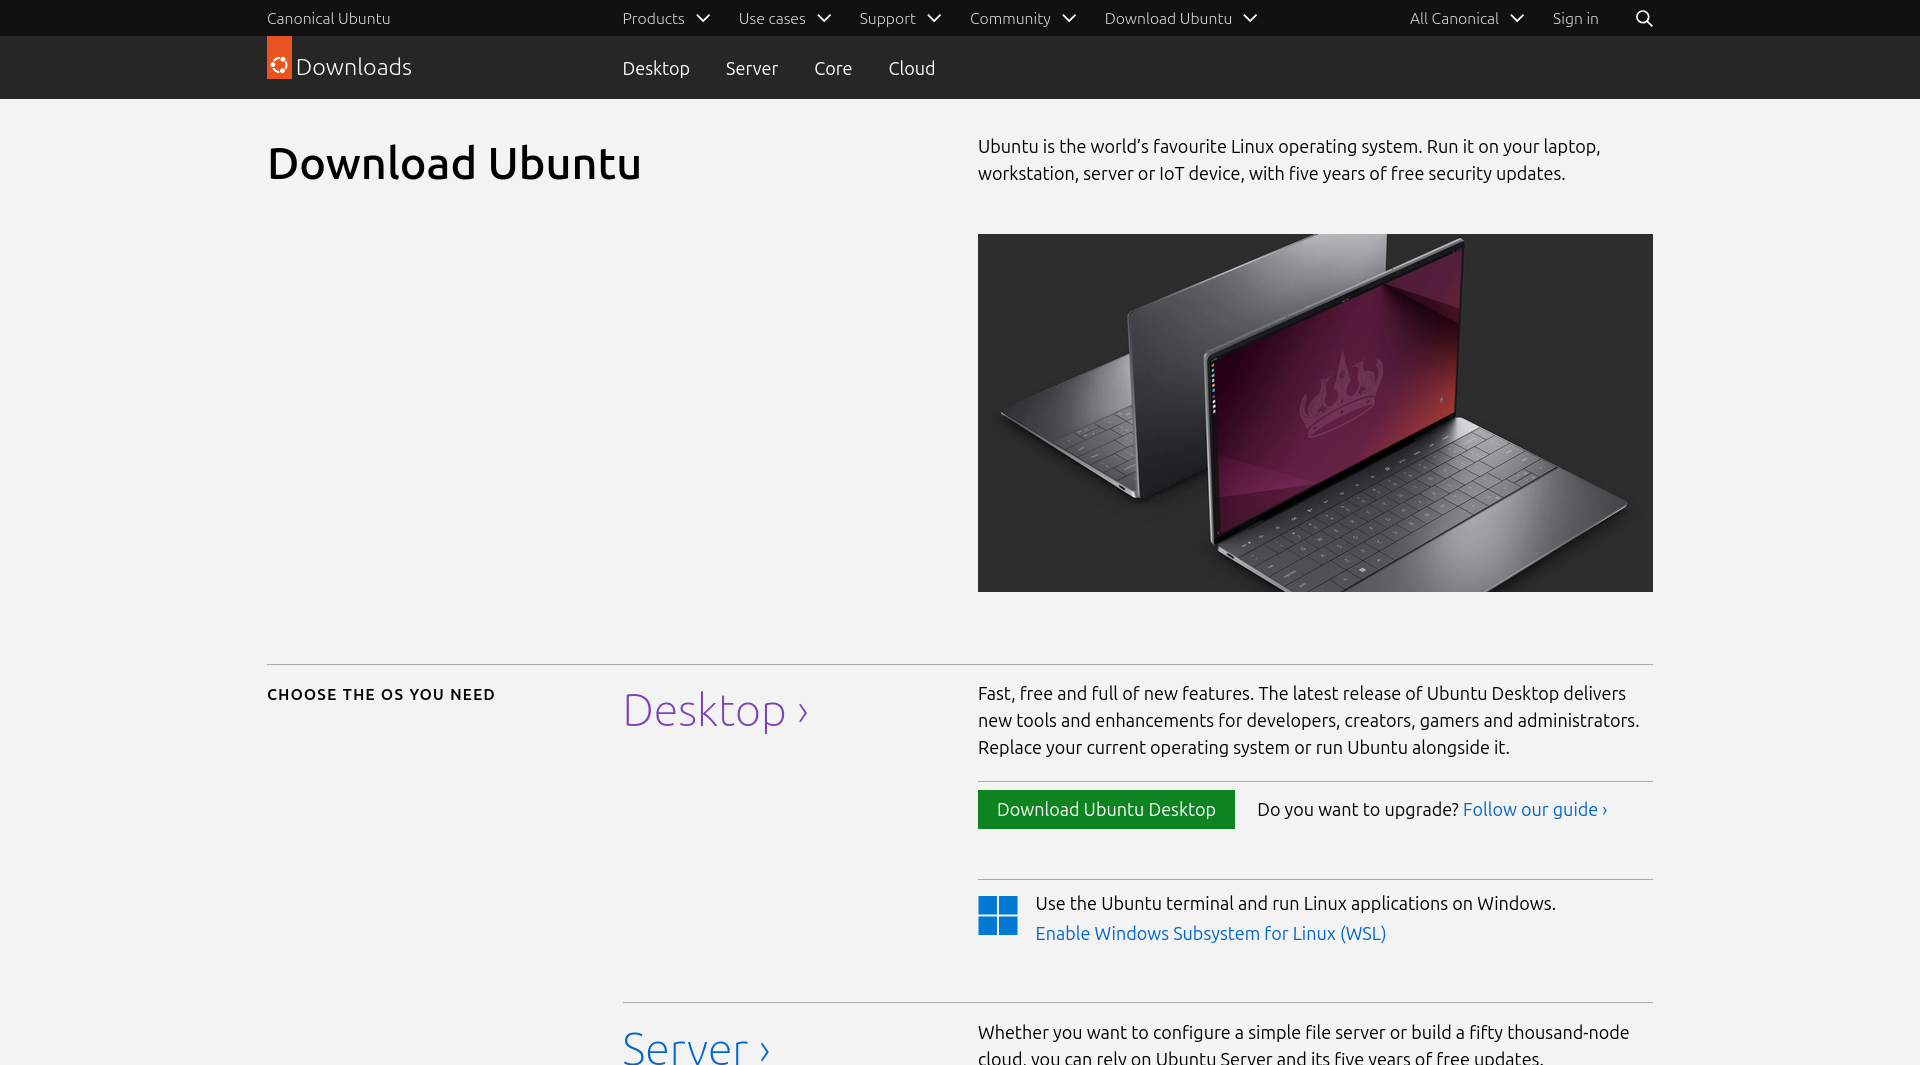
\includegraphics[width=0.80\linewidth]{./resources/images-ubuntu/web-ubuntu.png}
    \caption{Página oficial de Ubuntu}
\end{figure}

La descarga es cuanto menos sencilla. Haz clic en "Download Ubuntu Desktop" y selecciona la versión más actualizada.

Al terminar la descarga, deberíamos de tener en nuestro directorio de descargas un fichero como este:

\begin{figure}[H]
    \centering
    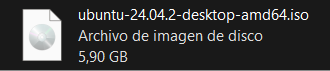
\includegraphics[width=0.40\linewidth]{./resources/images-ubuntu/descarga-iso.png}
    \caption{Imagen de disco de la instalación de Ubuntu}
\end{figure}

Esta es nuestra imagen de instalación. Existen formas de verificar que el fichero es el que dice ser y no una versión maliciosa, pero en la mayoría de casos, si estás descargando la imagen desde la página web oficial, no es necesario preocuparse.

Ya tenemos el fichero necesario. Sin embargo, mover el fichero a la unidad USB no es suficiente, primero hay que bootear la imagen.

\section{Booteando el medio de instalación}
Para instalar un sistema operativo se utiliza un medio de instalación externo (como un USB). Este medio de instalación tiene que ser capaz de ser ejecutado en el arranque del sistema, para que en vez de acceder al sistema operativo ya instalado, accedamos al instalador. A este proceso (de forma muy coloquial) se le llama booteo, y resulta ser bastante sencillo, al igual que el paso anterior.

Para bootear un medio necesitamos una utilidad de booteo. Existen varias opciones, pero una de las más utilizadas es Rufus, que además tiene licencia de Software Libre. Para instalarla, tenemos que acceder a la \href{https://rufus.ie/es/}{página web de Rufus}. Ve a la sección de descargas e instala una versión.

\begin{figure}[H]
    \centering
    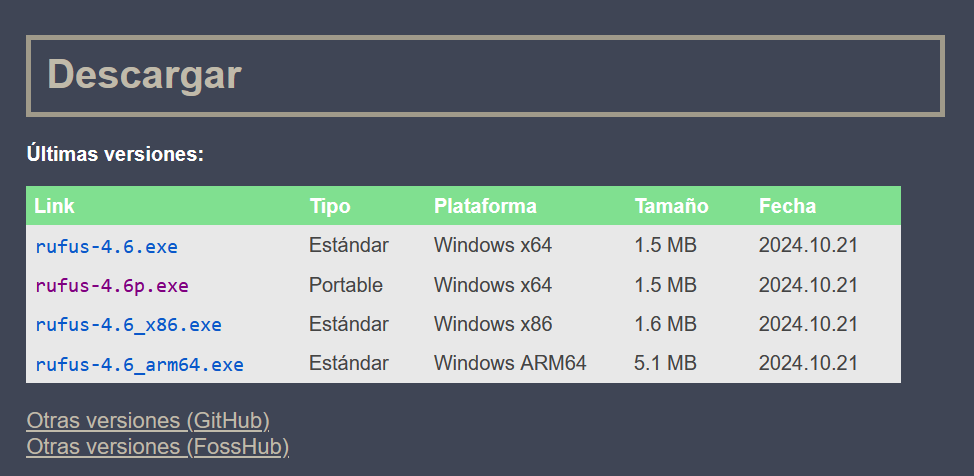
\includegraphics[width=0.75\linewidth]{./resources/images-ubuntu/rufus-versiones.png}
    \caption{Versiones disponibles de Rufus}
\end{figure}

El autor recomienda la versión portable, es muy ligera y no requiere instalación, basta con ejecutar el fichero ejecutable que obtendrás al descargarlo.

Así luce Rufus, como podemos ver es una interfaz bastante sencilla:

\begin{figure}[H]
    \centering
    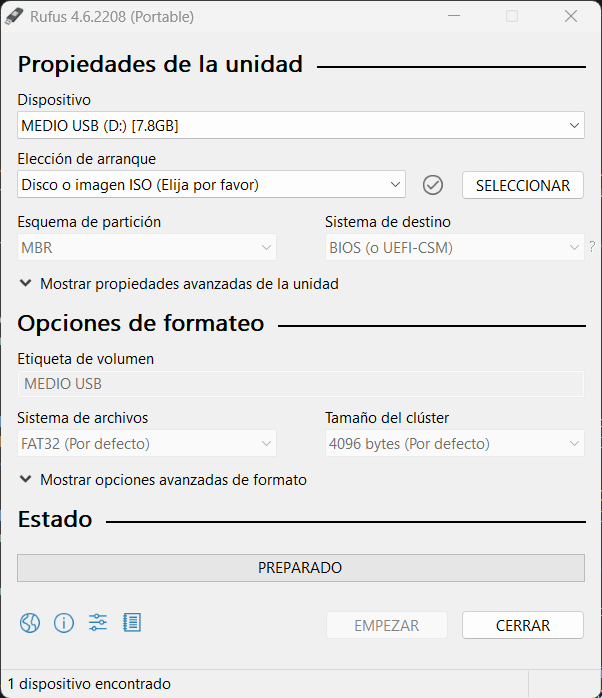
\includegraphics[width=0.75\linewidth]{./resources/images-ubuntu/rufus-interfaz.png}
    \caption{Interfaz de Rufus}
\end{figure}

Primero que nada, en la pestaña “Dispositivo”, tenemos que asegurarnos de que está seleccionado nuestro medio de instalación USB. Este va a ser el dispositivo que se va a formatear para que pueda ser booteable. Es decir, que se borrarán todos los datos. En mi caso, es la unidad D:, llamada “MEDIO USB”. Es de vital importancia que sea el dispositivo de almacenamiento externo el que esté seleccionado, ya que si está seleccionado nuestro disco duro interno, si bien se hará perfectamente booteable, perderemos todos los datos en éste, una conclusión no muy favorable.

Ahora tenemos que seleccionar la imagen de instalación que hemos descargado, la de Ubuntu. Para ello, le damos clic en “SELECCIONAR”, y buscamos el fichero .iso.

\begin{figure}[H]
    \centering
    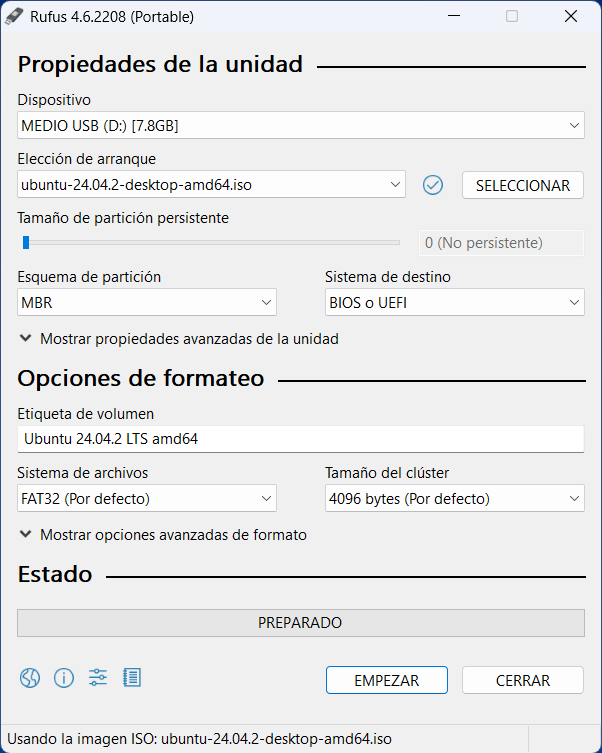
\includegraphics[width=0.75\linewidth]{./resources/images-ubuntu/rufus-iso-seleccionado.png}
    \caption{ISO de Ubuntu seleccionado}
\end{figure}

Veremos se desbloquean unas opciones nuevas, de las cuales no tenemos que modificar ninguna, es decir: La esquema de partición tiene que ser MBR, y el sistema de destino BIOS o UEFI. El formateo debe de ser FAT32 y el tamaño de cluster 4096 bytes. Una vez comprobados estos parámetros, podemos darle al botón “EMPEZAR”.

\begin{figure}[H]
    \centering
    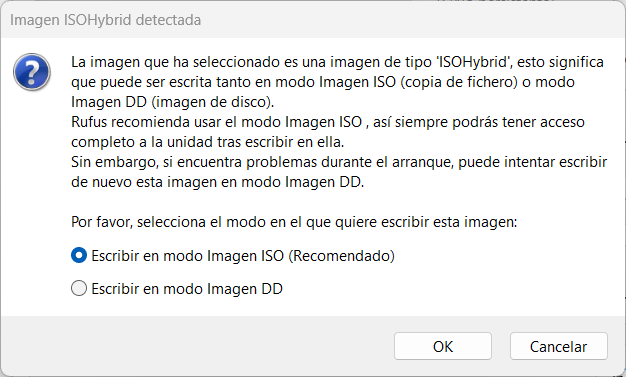
\includegraphics[width=0.5\linewidth]{./resources/images-ubuntu/rufus-tipo-iso-prompt.png}
    \caption{Aviso sobre el tipo de ISO}
\end{figure}

\begin{figure}[H]
        \centering
        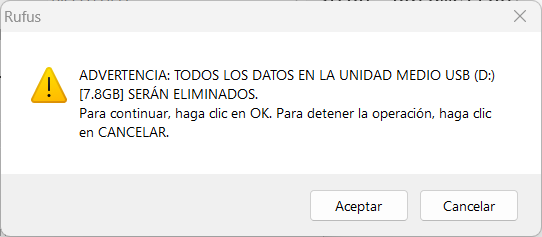
\includegraphics[width=0.5\linewidth]{./resources/images-ubuntu/rufus-formateo.png}
        \caption{Advertencia sobre la pérdida de datos de la unidad}
\end{figure}

Nos saldrán estos dos prompts. En el primero, selecciona el modo Imagen ISO, y una vez leída la advertencia de la segunda ventana, dale clic en Aceptar. Este proceso llevará un rato, ya que la imagen de instalación de Ubuntu es bastante pesada. Cuando termine, no olvides retirar el hardware con seguridad (si Rufus no lo ha hecho ya), y guardarlo para más tarde. Mientras que esperas, puedes empezar con el siguiente paso de la instalación.

\chapter{Creando espacio libre en nuestro disco}

\textbf{NOTA}: Ignora este capítulo si deseas eliminar Windows en su totalidad y tener solo Ubuntu instalado en tu sistema.

Para asignarle un espacio a Ubuntu en nuestro sistema, primero tenemos que generar una partición con espacio libre. En un equipo con Windows instalado por defecto, la instalación inicial asigna todo su espacio a Windows. No obstante, tenemos herramientas para generar espacio libre.

\section{El administrador de discos}

Abre el menú de inicio y busca “Administración de discos” y ejecuta el programa del resultado de la búsqueda.

\begin{figure}[H]
    \centering
    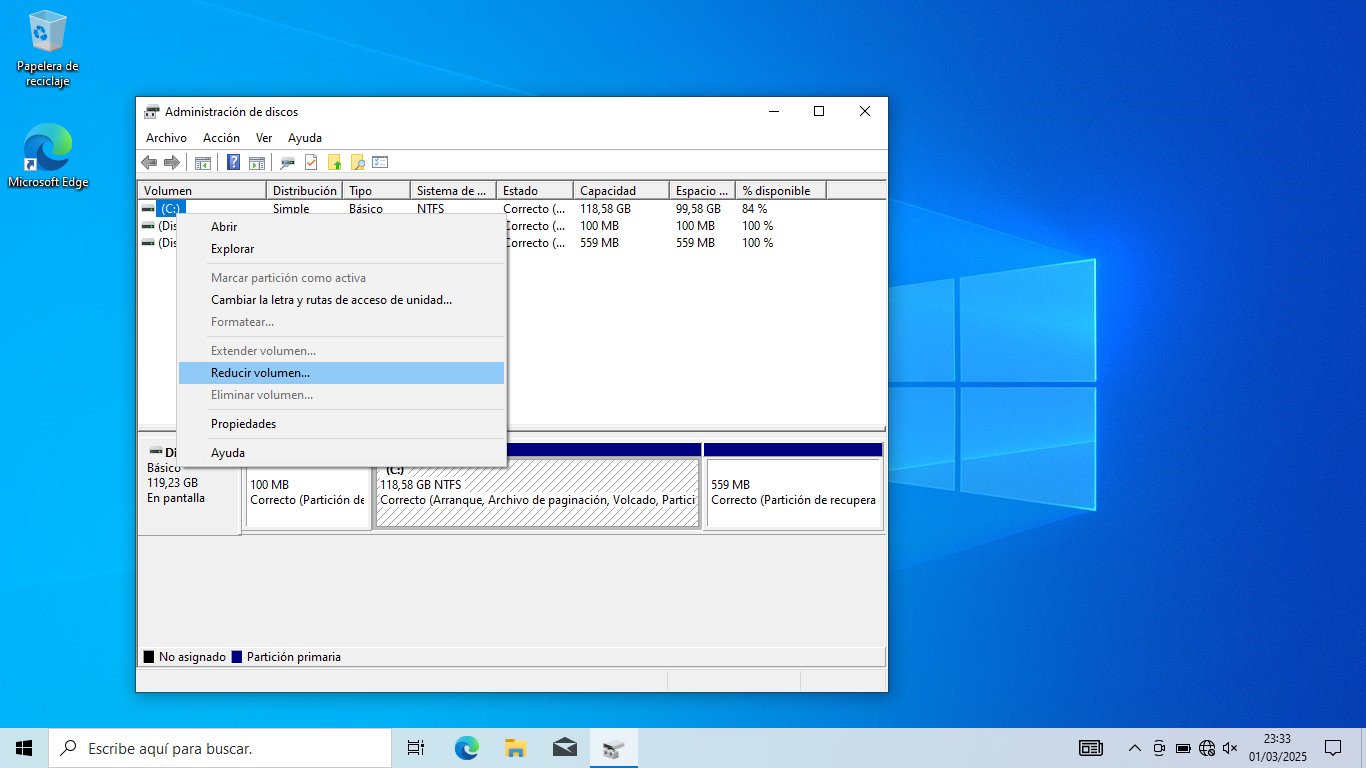
\includegraphics[width=0.80\linewidth]{./resources/images-ubuntu/administrador-discos.png}
    \caption{Interfaz del administrador de discos}
\end{figure}

Se nos abrirá esta interfaz. Con este programa, podemos modificar el tamaño de las particiones de nuestro disco. Como podemos aumentar tanto como reducir el tamaño (dentro de lo que nos lo permita el espacio de almacenamiento total de nuestro disco duro), si reducimos el espacio de la partición principal de Windows, generaremos espacio libre que Ubuntu podrá utilizar.

Busca la partición principal del sistema. Normalmente es la que tiene la letra de acceso a unidad “C:”, o la que más espacio de almacenamiento tiene. Selecciónala, haz clic derecho en ella, y luego haz clic en reducir volumen. Se nos abrirá el siguiente menú:

\begin{figure}[H]
    \centering
    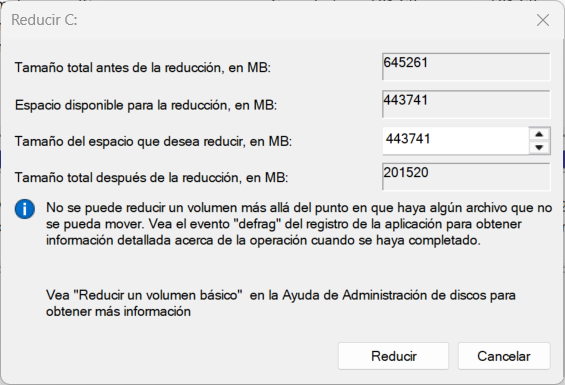
\includegraphics[width=0.75\linewidth]{./resources/images-ubuntu/administrador-discos-reducir-volumen.png}
    \caption{Interfaz de reducción de volumen}
\end{figure}

Con este menú podemos reducir el tamaño de nuestra partición principal. En el tercer cuadro numérico (el del tamaño del espacio que deseamos reducir), esencialmente tenemos que introducir la cantidad de espacio que le vamos a quitar a Windows para entregárselo a Ubuntu, en MB. Por ejemplo, si queremos que nuestro sistema operativo de Ubuntu tenga 80 GB de almacenamiento, deberíamos introducir “80000”. Luego, le damos clic a “Reducir”.

\begin{figure}[H]
    \centering
    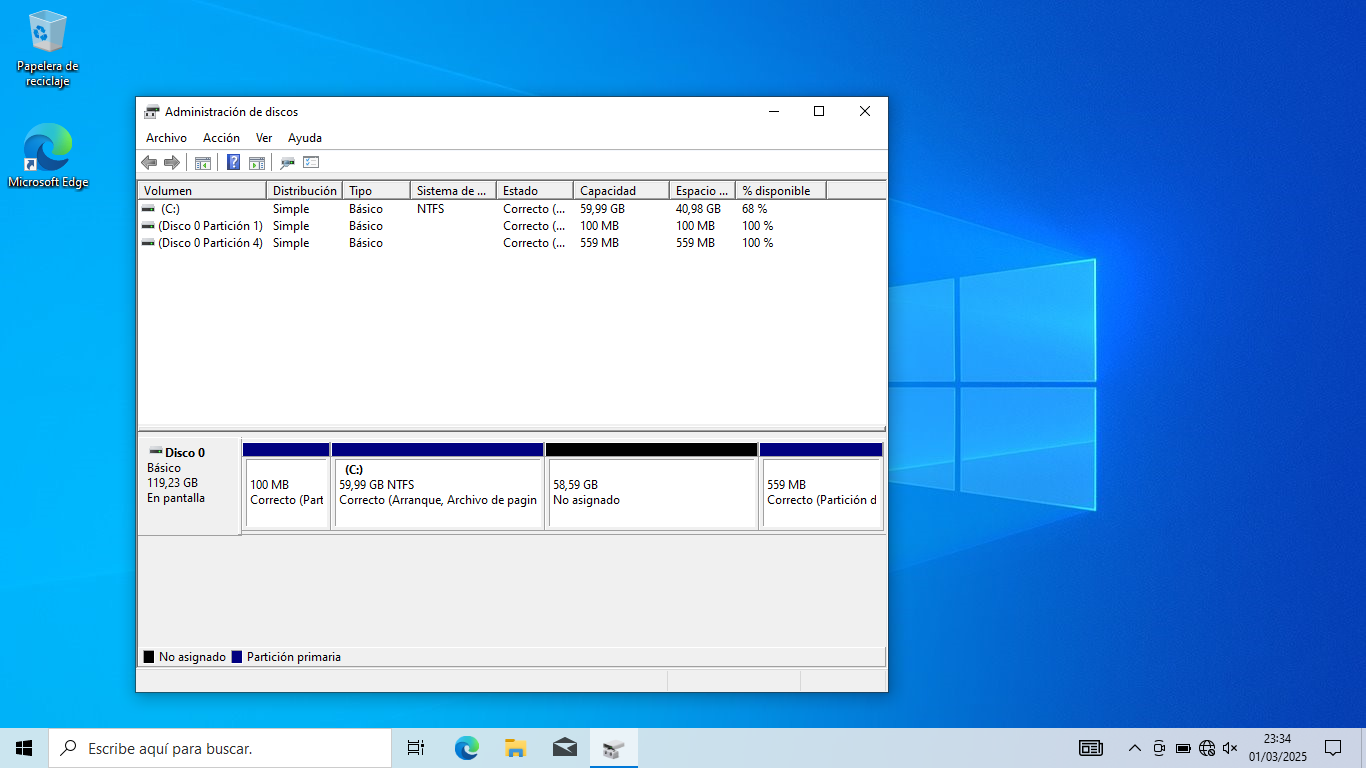
\includegraphics[width=0.85\linewidth]{./resources/images-ubuntu/administrador-discos-creado.png}
    \caption{Espacio libre creado}
\end{figure}

Ya hemos “hecho hueco” en nuestro sistema para instalar Ubuntu (En mi caso, le he asignado 60 gigas por falta de almacenamiento). Ahora, ya podemos apagar nuestro equipo para comenzar la instalación en sí.

\chapter{Arrancando el sistema en la instalación}

Ahora que tenemos nuestro medio de instalación listo para ser booteado, tenemos que hacer unos preparativos para ejecutarlo. Para ello, vamos a acceder a la BIOS/UEFI de nuestro sistema, un área de solo lectura que nos permite configurar cómo se comporta nuestro sistema en el arranque.

Para empezar, inserta la unidad USB antes de encender tu equipo. Una vez hecho eso, busca en internet cómo acceder a la BIOS/UEFI de tu sistema. Dependiendo de la marca y el modelo, la forma de acceder puede variar, pero normalmente las teclas suelen ser F2 o F12. Asegurándote de que el USB está conectado, enciende el sistema y accede a la BIOS/UEFI. Se nos abrirá un menú, que en función de la marca y modelo de tu ordenador tendrá un diseño u otro. Aquí tienes un ejemplo:

\begin{figure}[H]
    \centering
    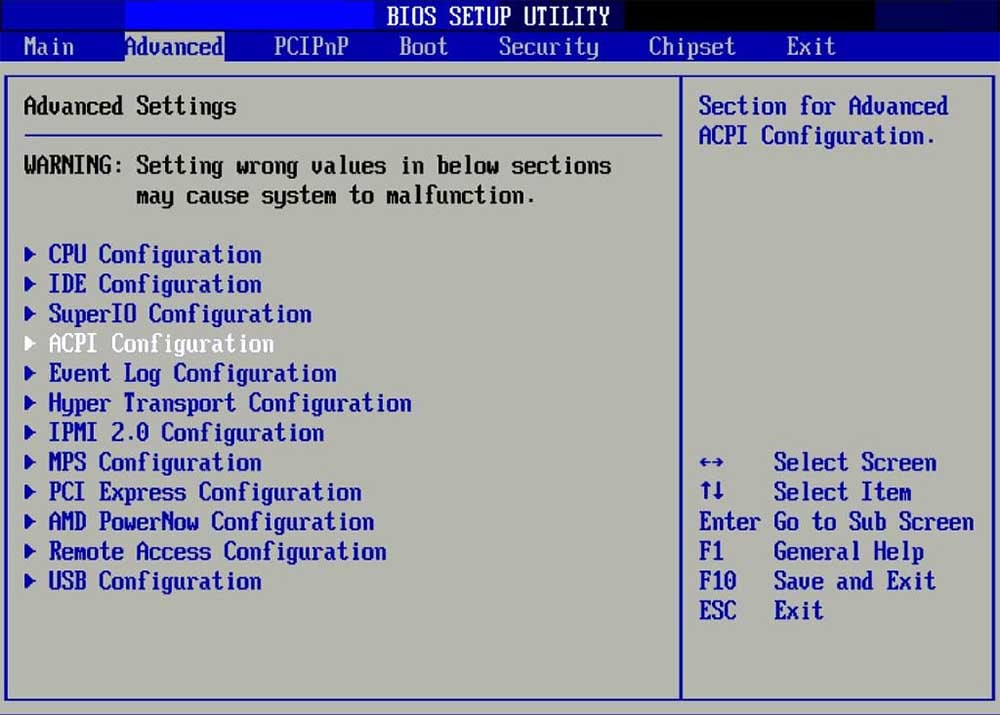
\includegraphics[width=0.80\linewidth]{./resources/images-ubuntu/ejemplo-bios.jpg}
    \caption{Ejemplo genérico de una BIOS/UEFI}
\end{figure}

De todas las pestañas de la BIOS/UEFI, nos interesa la de “Boot”.

\begin{figure}[H]
    \centering
    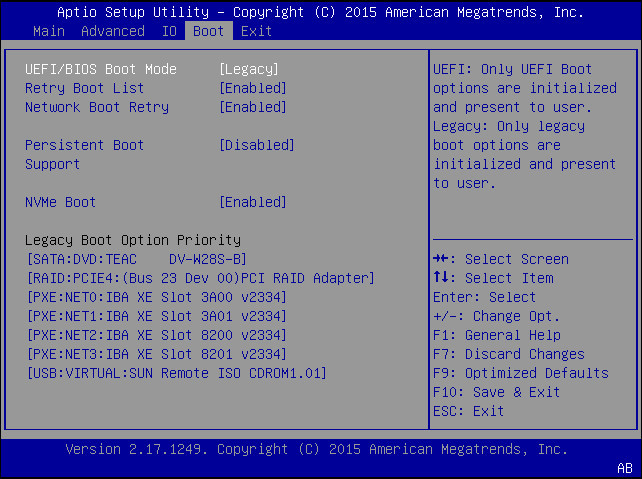
\includegraphics[width=0.80\linewidth]{./resources/images-ubuntu/bios-boot.jpg}
    \caption{Sección de boot}
\end{figure}

En esta pestaña, entre otras cosas, podemos configurar qué arranque se va a ejecutar al iniciar el sistema. Normalmente el primero será tu disco duro, que en él tiene el Windows Boot Manager. En esta situación, no queremos que se ejecute ese, queremos que se ejecute nuestra unidad USB al arrancar el sistema (que debería de aparecer como opción si la tenemos conectada), así que tenemos que seleccionarla y moverla al primer puesto (la forma de hacer este paso varía en función de los controles de tu BIOS/UEFI, pero normalmente las instrucciones de uso son visibles en pantalla). Una vez modificado el orden de arranque, podemos guardar la configuración y reiniciar el sistema.

\chapter{Instalación de Ubuntu}

Si hasta ahora has seguido las instrucciones correctamente, al reiniciar el sistema habrá arrancado el medio de instalación de Ubuntu. La primera ventana que veremos será la de GRUB, parecida (si no igual) a esta:

\begin{figure}[H]
    \centering
    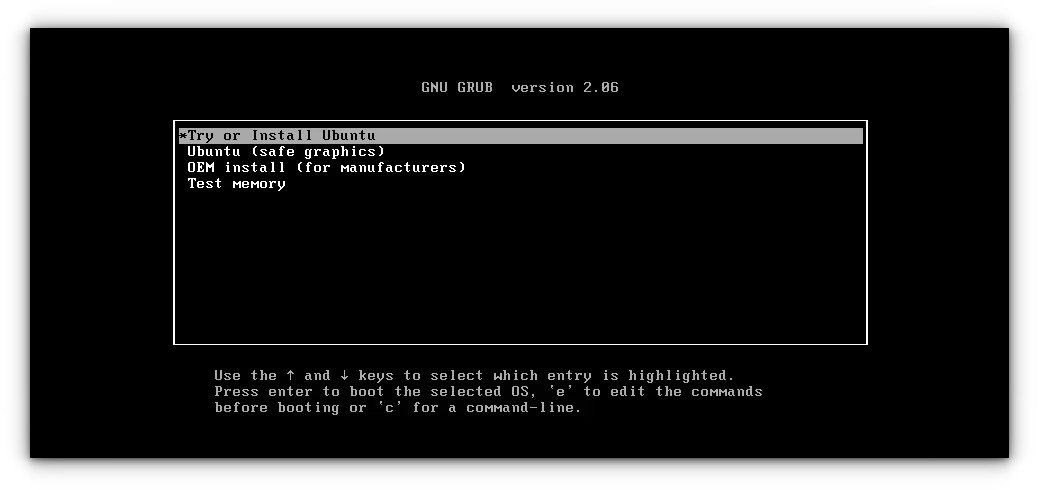
\includegraphics[width=0.85\linewidth]{./resources/images-ubuntu/grub.png}
    \caption{Interfaz de GRUB}
\end{figure}

Le damos a enter en “Try or Install Ubuntu”, y a partir de aquí nos encontraremos con interfaces más amigables.

\begin{figure}[H]
    \centering
    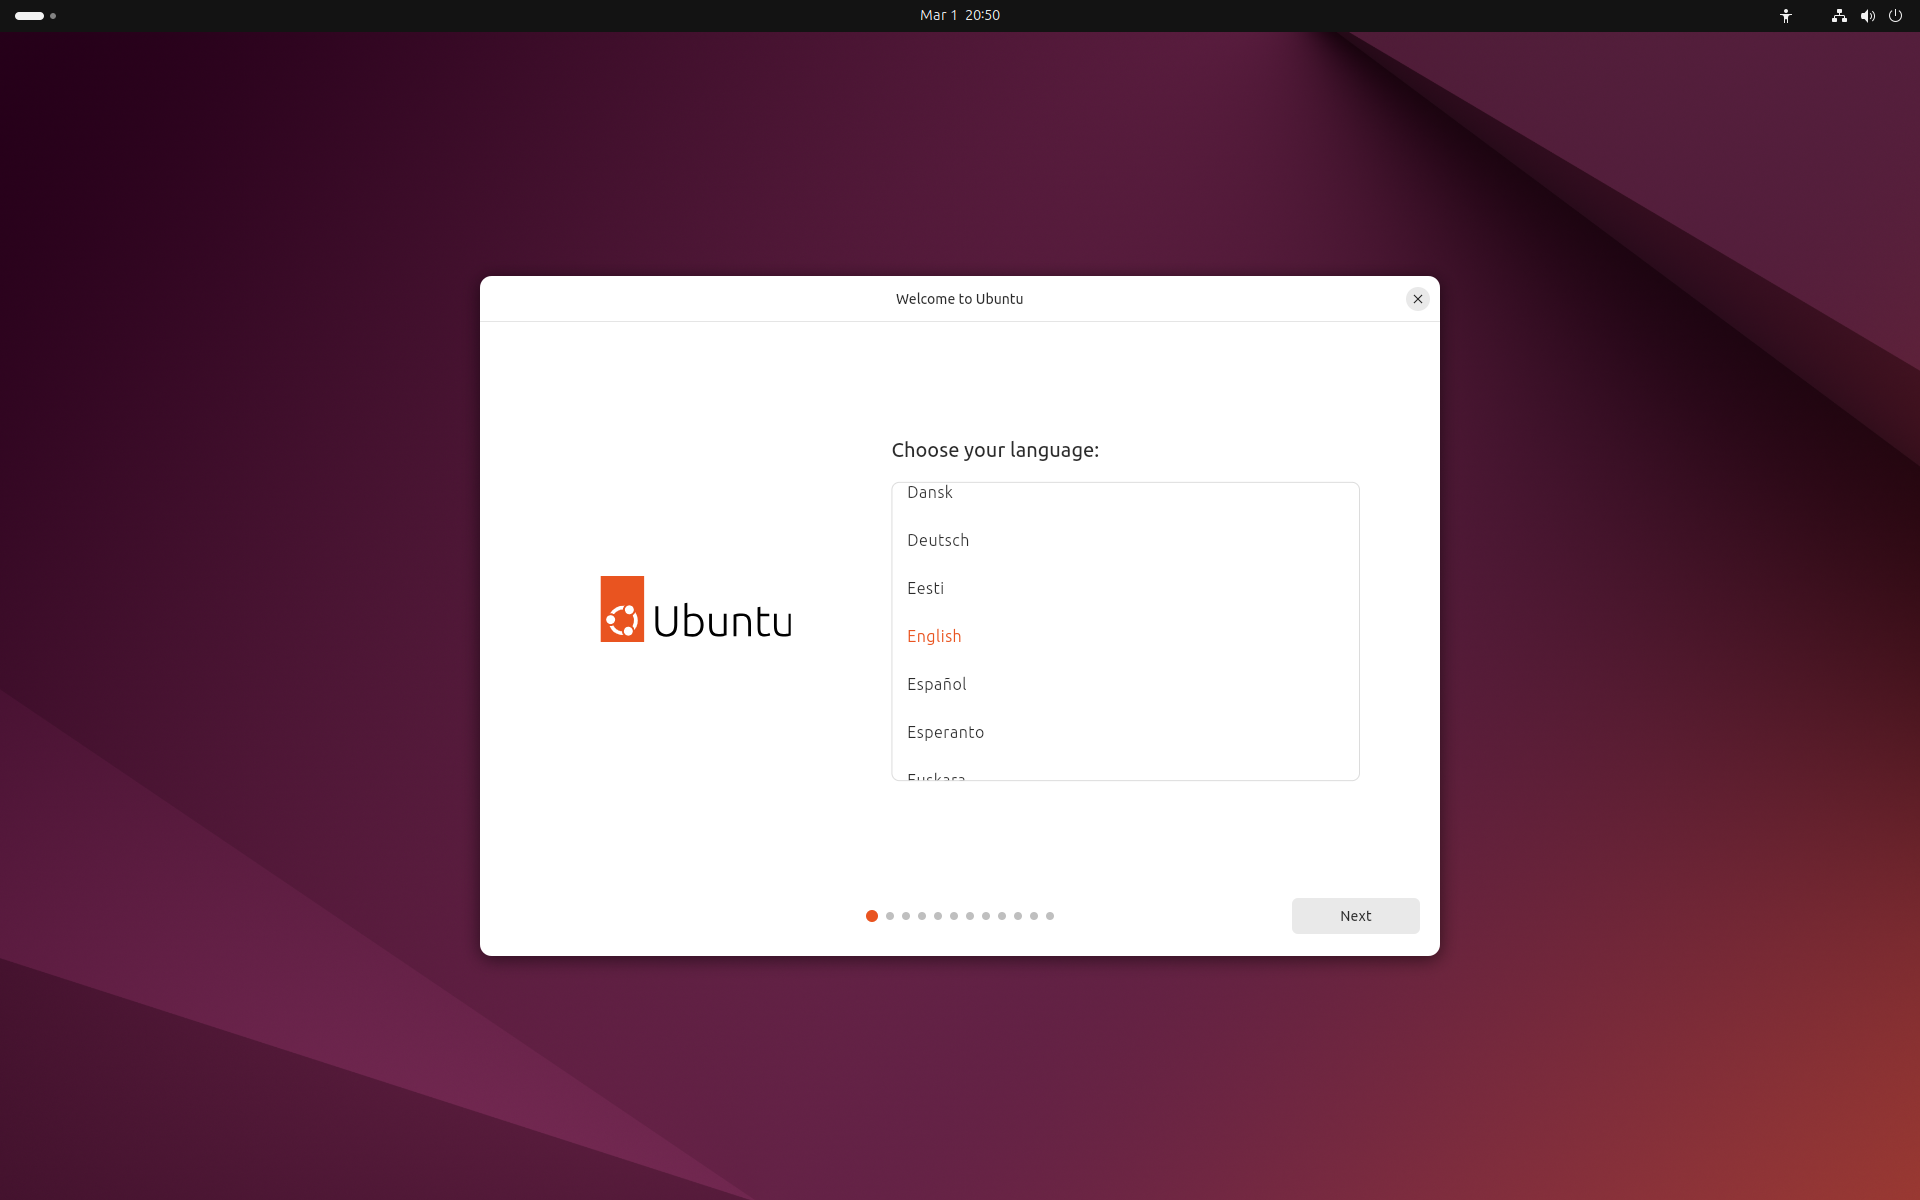
\includegraphics[width=0.85\linewidth]{./resources/images-ubuntu/ubuntu-lenguaje.png}
    \caption{Selección de lenguaje de Ubuntu y primer paso de la instalación}
\end{figure}

Este es el instalador de Ubuntu. A partir de aquí, la instalación no es mucho más complicada que la de cualquier programa en Windows. En cualquier caso, iremos paso a paso. 

Antes de continuar, cabe destacar una propiedad interesante del instalador de Ubuntu (y el de otras distribuciones de Linux). El instalador realmente es un mini-sistema operativo, es decir, cumple las funcionalidades básicas de un sistema operativo normal. Antes de hacer nada, dedícale un momento a cerrar el instalador y ver qué pasa:

\begin{figure}[H]
    \centering
    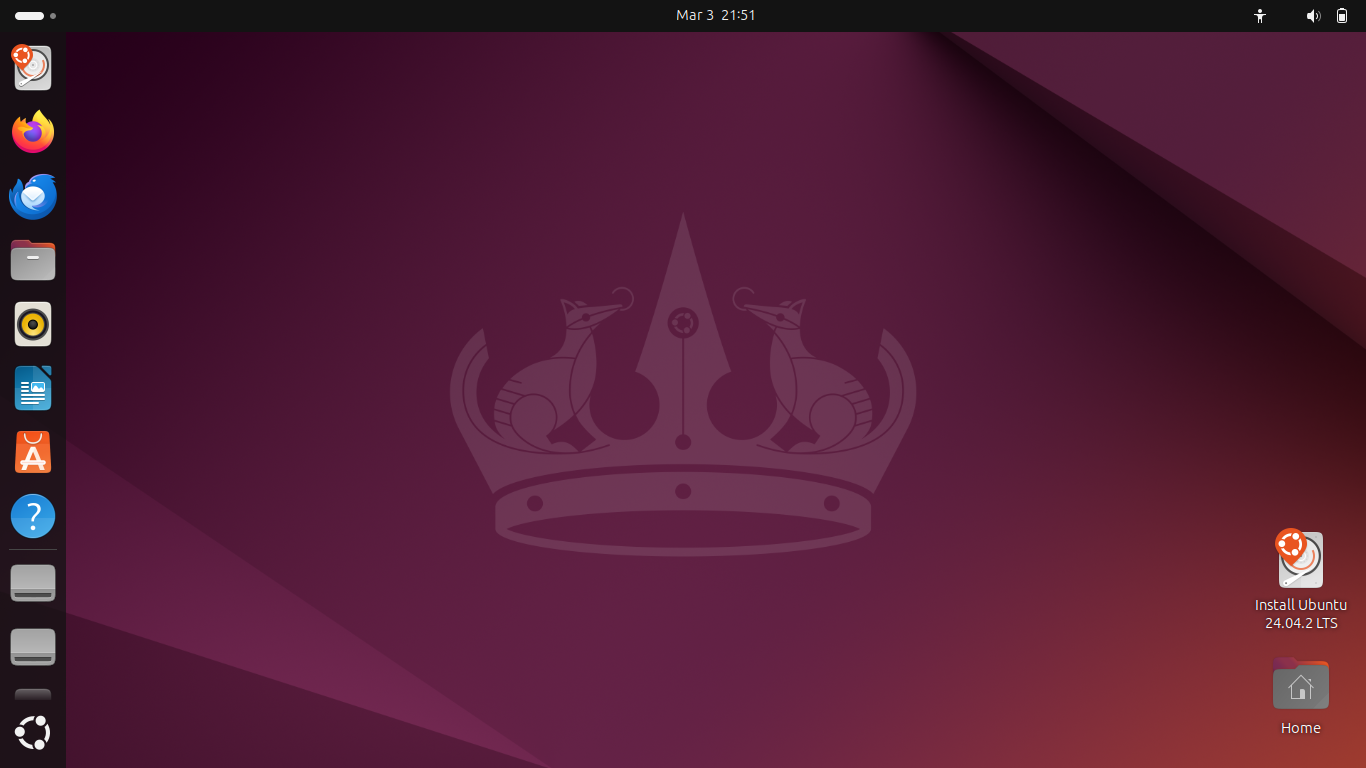
\includegraphics[width=0.85\linewidth]{./resources/images-ubuntu/escritorio-ubuntu.png}
    \caption{Escritorio de Ubuntu}
\end{figure}

Como puedes ver, este es el escritorio de Ubuntu, en el que podemos acceder a varias funcionalidades de la distribución:

\begin{figure}[H]
    \centering
    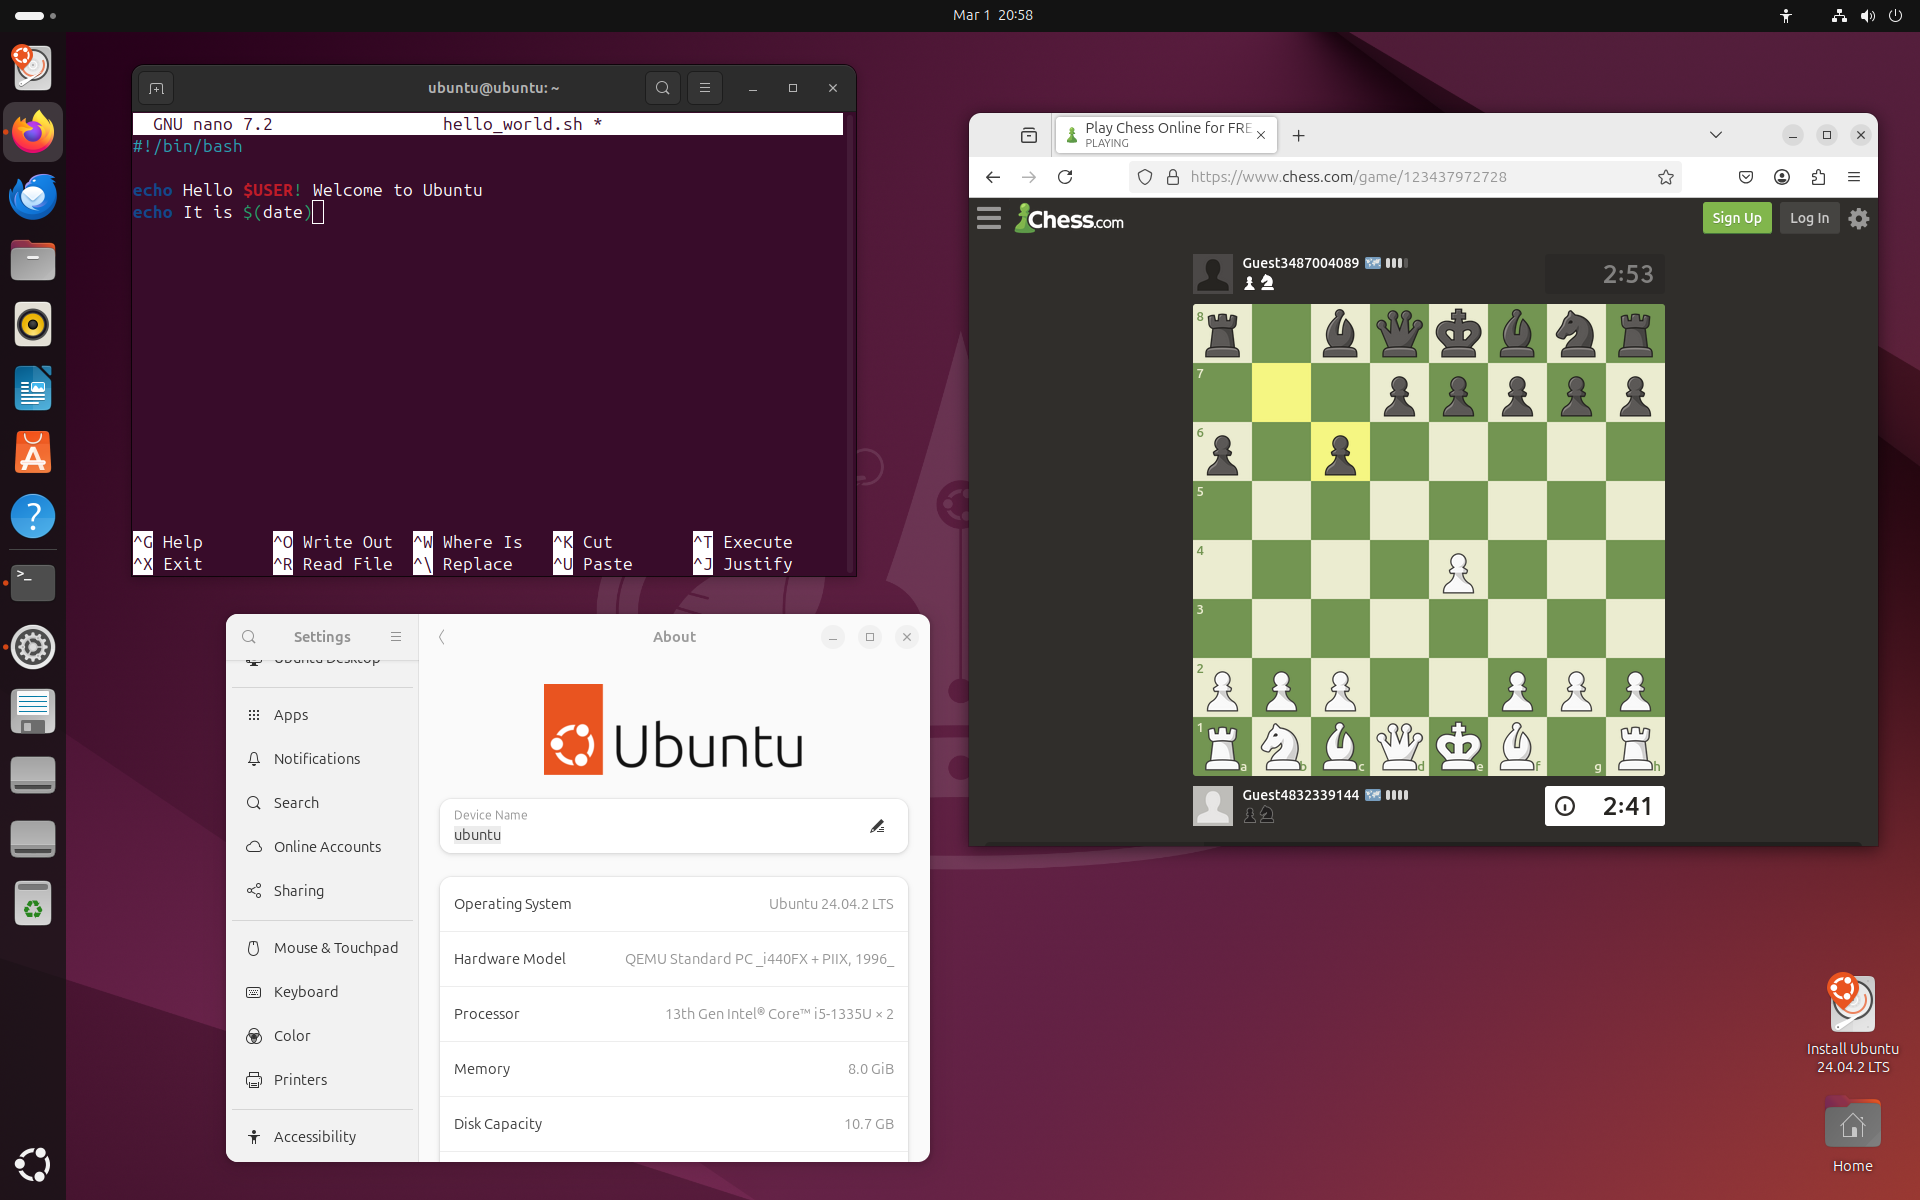
\includegraphics[width=0.85\linewidth]{./resources/images-ubuntu/ubuntu-tareas.png}
    \caption{Realización de diferentes tareas en la distribución}
\end{figure}


En esta captura estoy ejecutando diferentes tareas que se podrían ejecutar perfectamente en un sistema operativo ya instalado. Esto lo hace Ubuntu para que puedas probar su distribución sin necesariamente instalarla.

Sin embargo, tiene otra funcionalidad muy importante. Te da acceso a una terminal:

\begin{figure}[H]
    \centering
    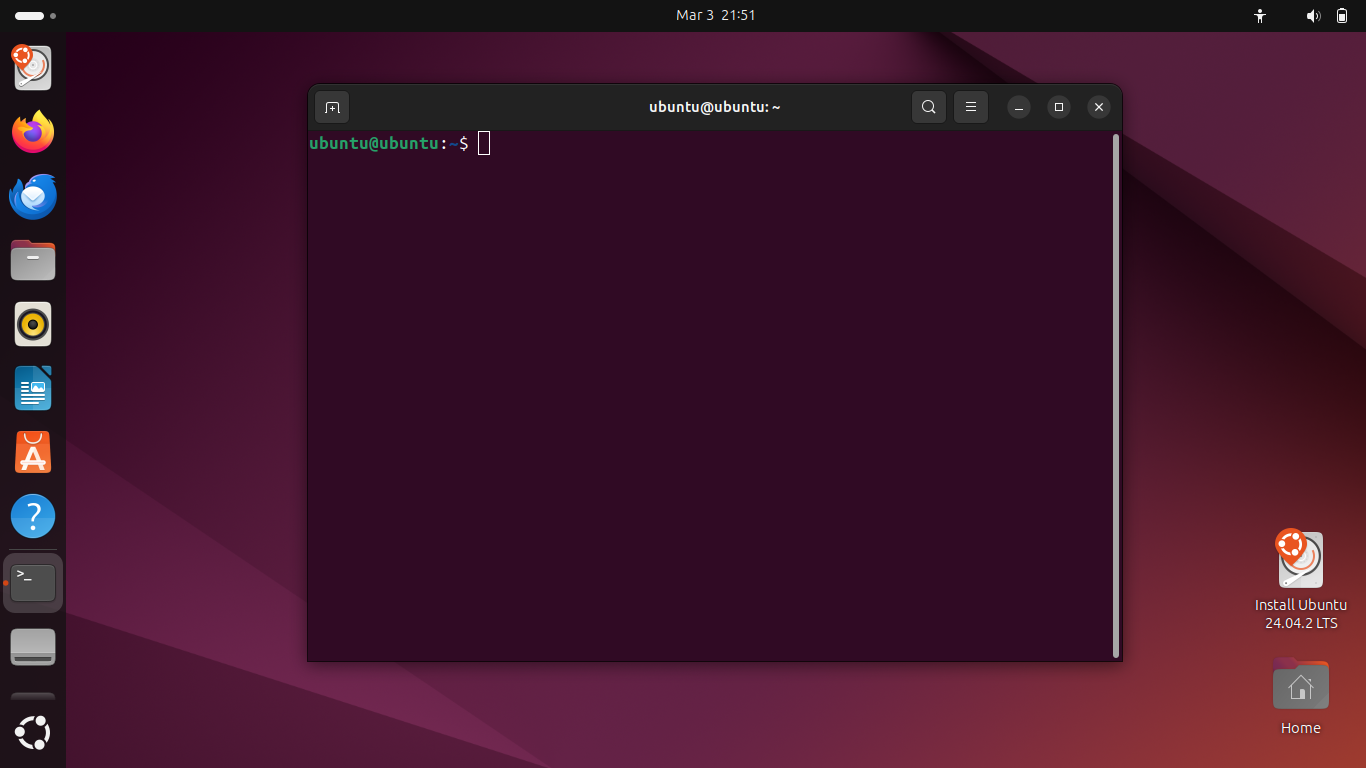
\includegraphics[width=0.85\linewidth]{./resources/images-ubuntu/ubuntu-terminal.png}
    \caption{Terminal de Ubuntu}
\end{figure}

Esto implica que puedes ejecutar comandos de la terminal fuera del entorno del sistema operativo ya instalado, es decir, que puedes tener un acceso “remoto” a tu sistema operativo desde un entorno de instalación. Para conseguir esto haría falta montar las particiones de tu disco en el medio de instalación, algo que no veremos en esta guía. Pero debes de quedarte con la idea de que un medio de instalación puede servir como un sistema de recuperación de tu sistema operativo, que puede ser de gran utilidad si (por la razón que sea) pierdes acceso a tu sistema. Solamente recuerda que el contenido del medio de instalación se reiniciará en cada apagado. En cualquier caso, continuemos con la instalación.

\begin{figure}[H]
    \centering
    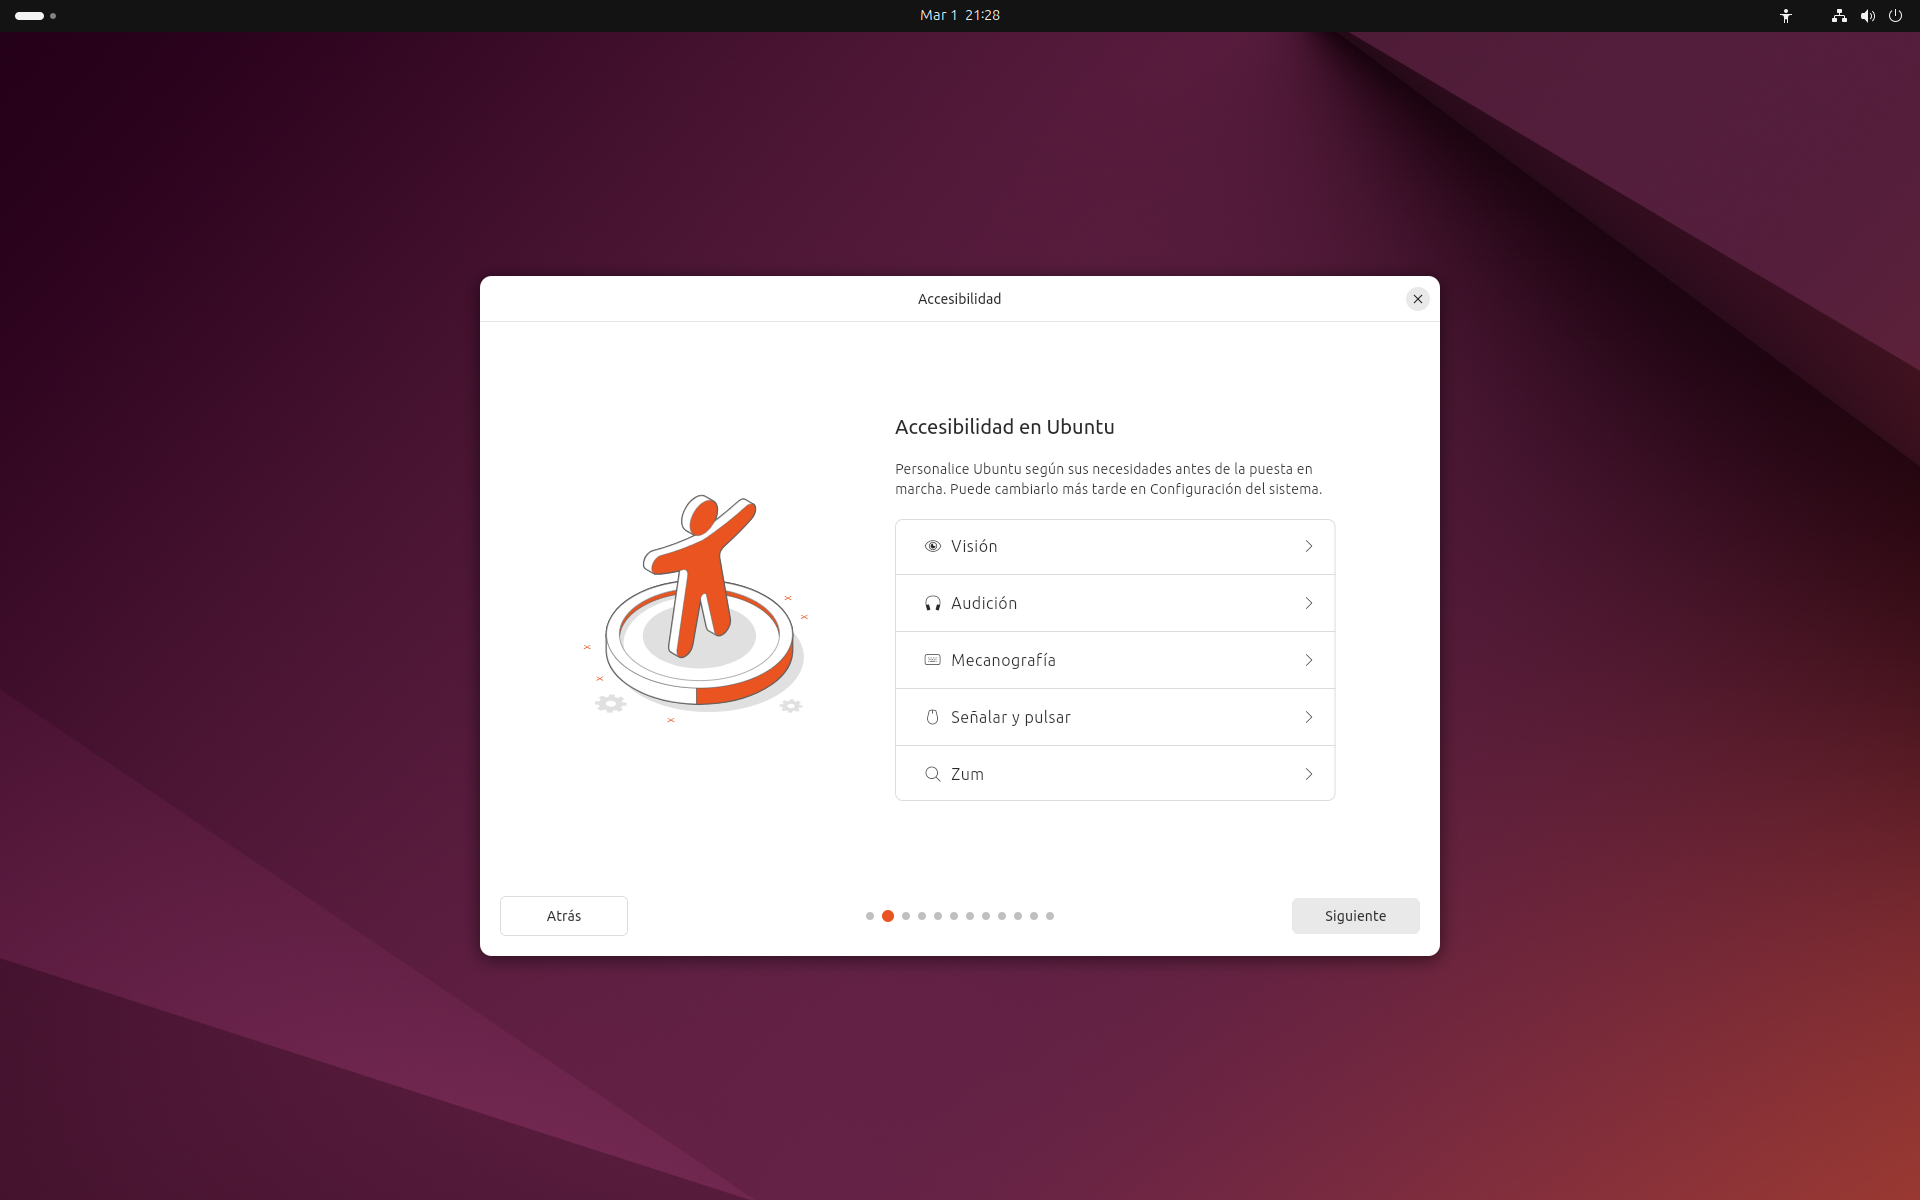
\includegraphics[width=0.85\linewidth]{./resources/images-ubuntu/ubuntu-accesibilidad.png}
    \caption{Seccion de accesibilidad}
    \label{fig:placeholder}
\end{figure}

Al seleccionar el idioma, te preguntarán sobre tus necesidades de accesibilidad. Si requieres alguna de estas ayudas, selecciónalas acorde a tus necesidades y continúa con el siguiente paso.

\begin{figure}[H]
    \centering
    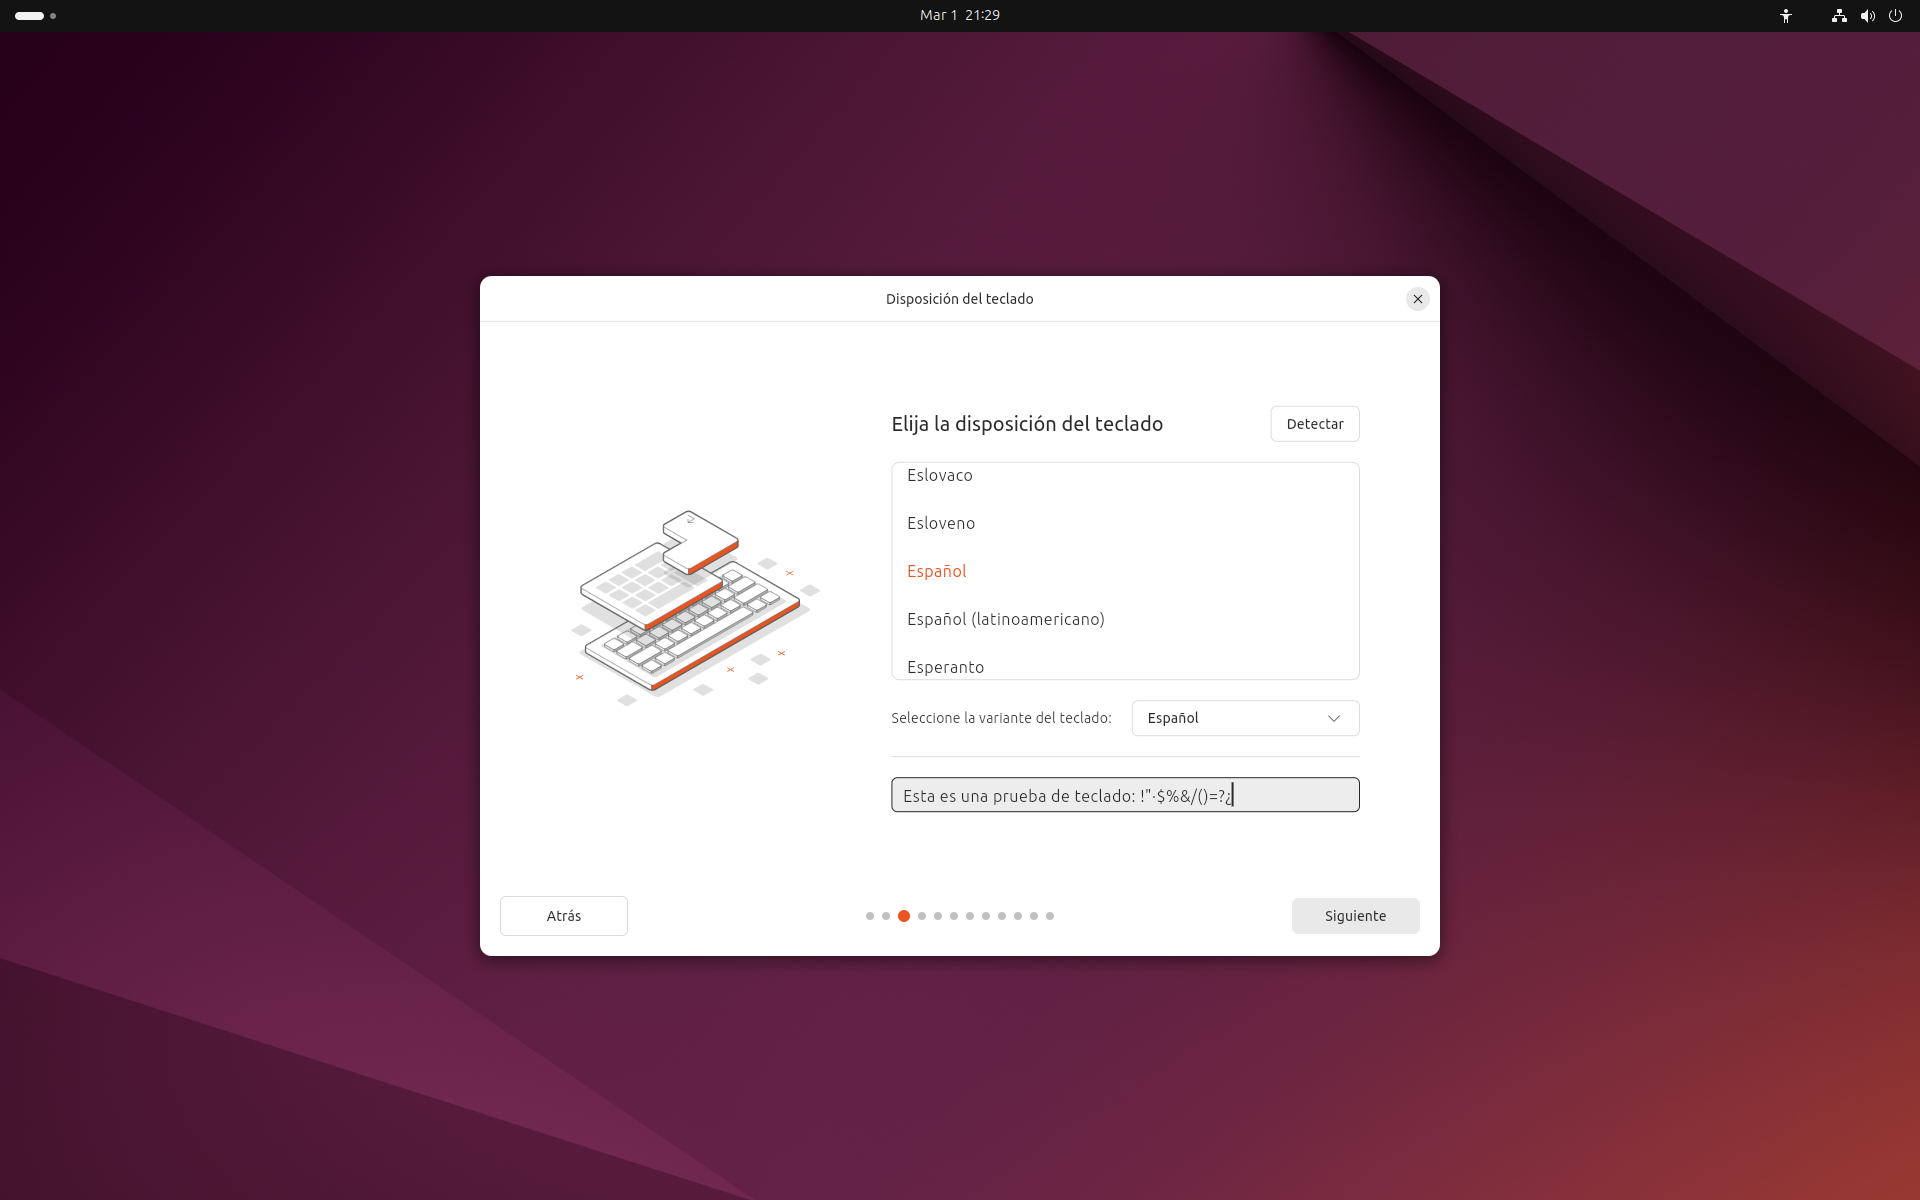
\includegraphics[width=0.85\linewidth]{./resources/images-ubuntu/ubuntu-teclado.png}
    \caption{Opciones de distribución de teclado}
\end{figure}


Algo que vas a querer tener configurado desde el principio es la distribución de tu teclado. Selecciona la adecuada en la lista o usa la opción inteligente de “Detectar” si tienes dudas. El instalador te deja un cuadro de texto para probar tu distribución actual.

\begin{figure}[H]
    \centering
    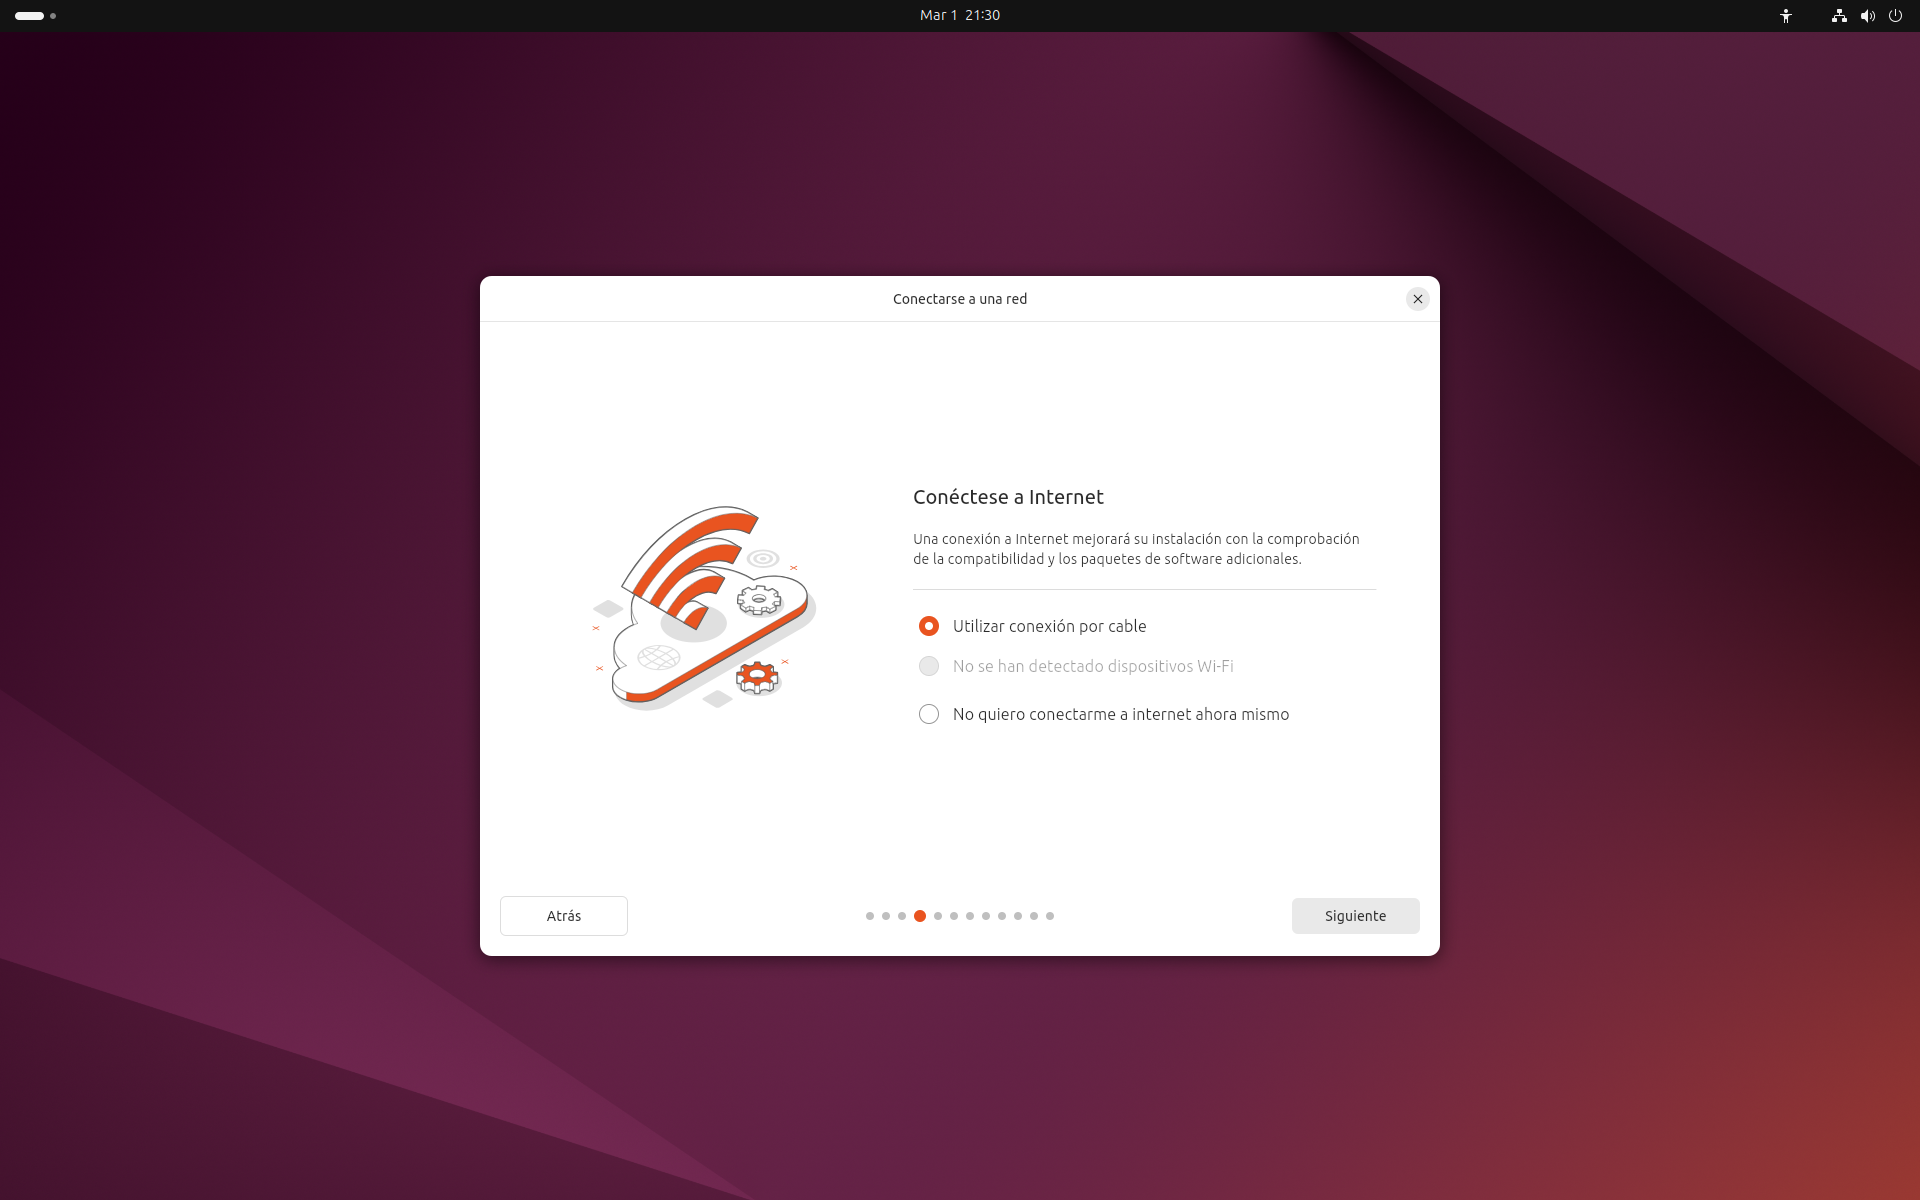
\includegraphics[width=0.85\linewidth]{./resources/images-ubuntu/ubuntu-internet.png}
    \caption{Configuración de internet}
\end{figure}

El siguiente paso es configurar tu conexión a internet (si lo deseas, no es obligatoria durante la instalación). En mi caso, como estaba ejecutando la instalación en una máquina virtual, la única opción que tenía disponible era mediante cable ethernet. En caso de que necesites conectarte mediante conexión Wi-Fi, selecciona la opción y sigue las instrucciones. El procedimiento es muy similar a cómo lo harías en un teléfono móvil.

\begin{figure}[H]
        \centering
        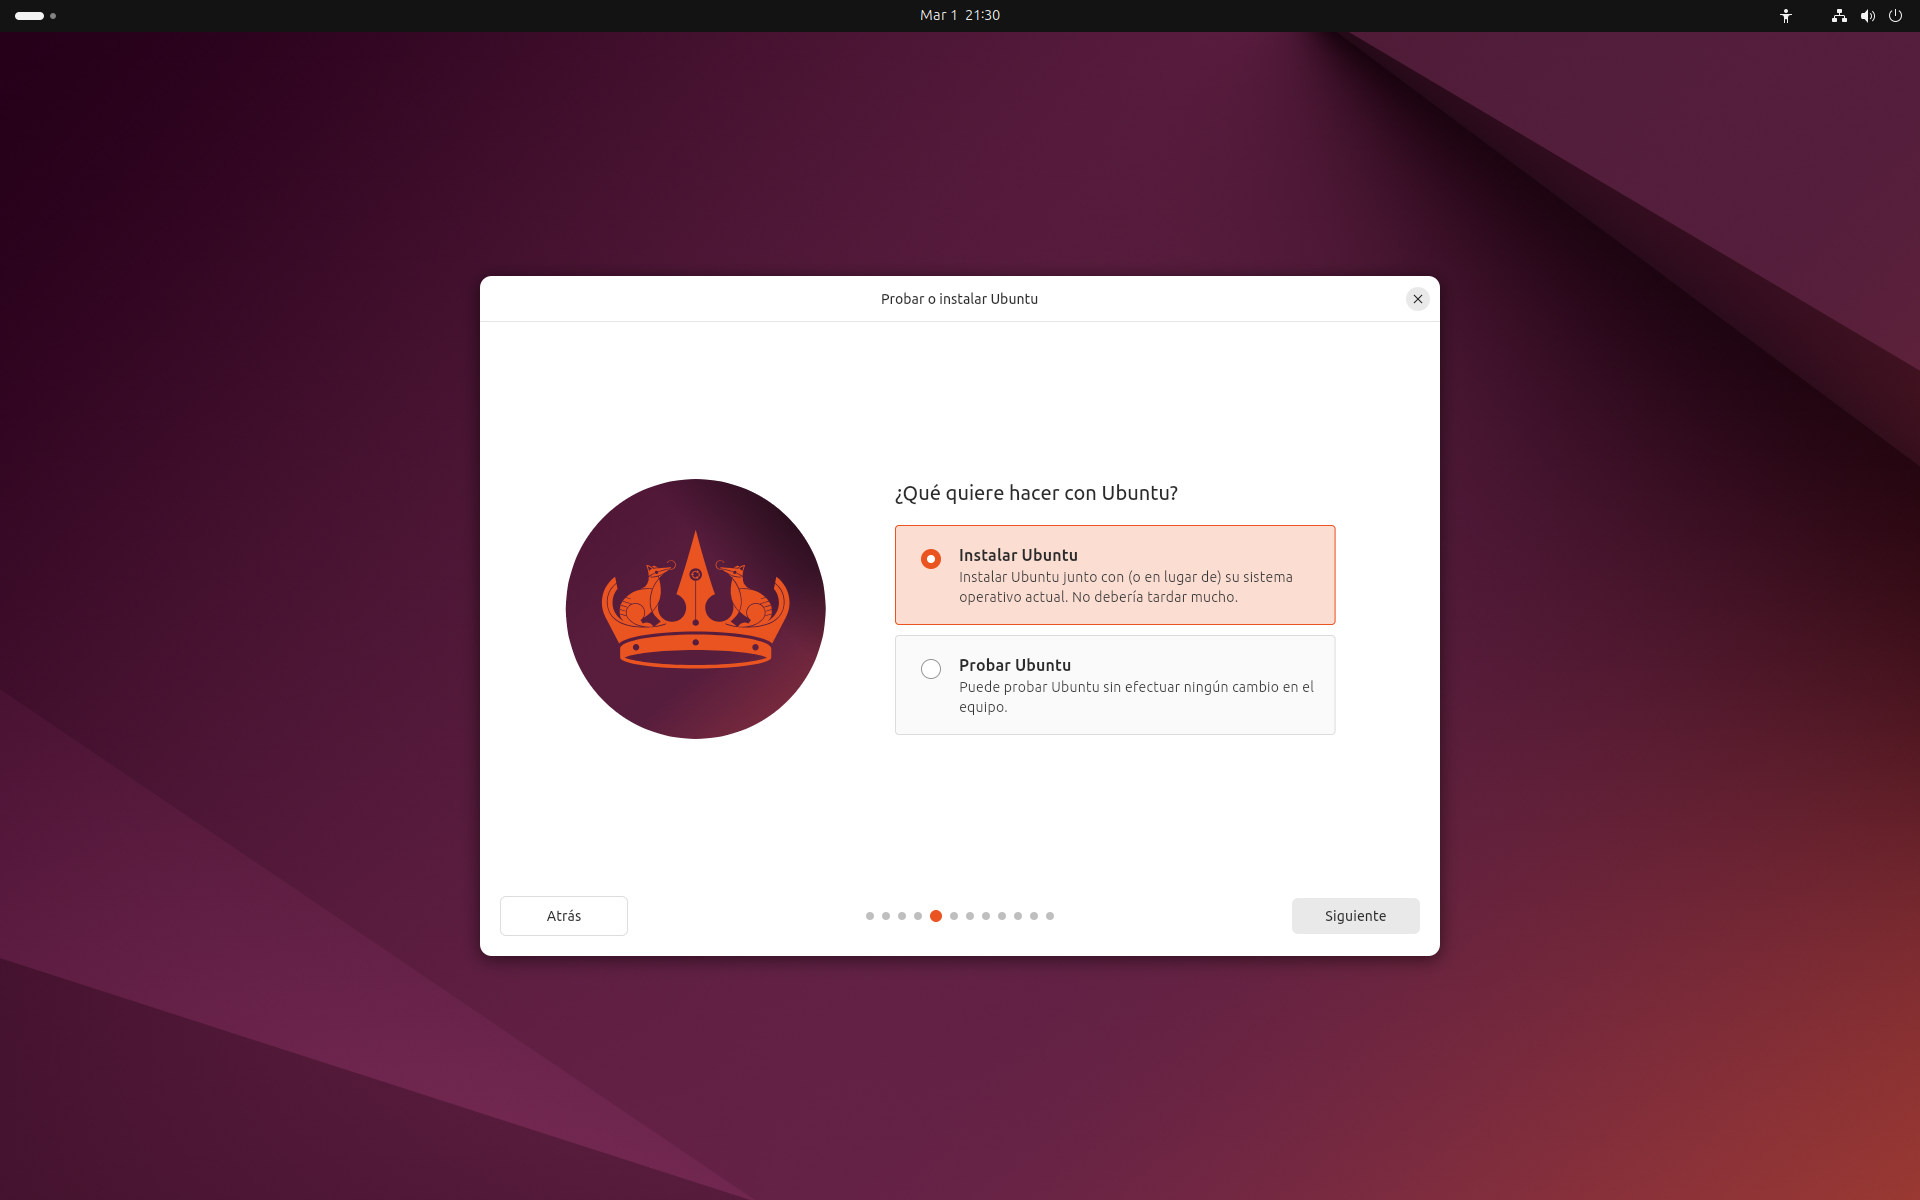
\includegraphics[width=0.85\linewidth]{./resources/images-ubuntu/ubuntu-instalacion.png}
        \caption{Elección de instalación}
\end{figure}

\begin{figure}[H]
        \centering
        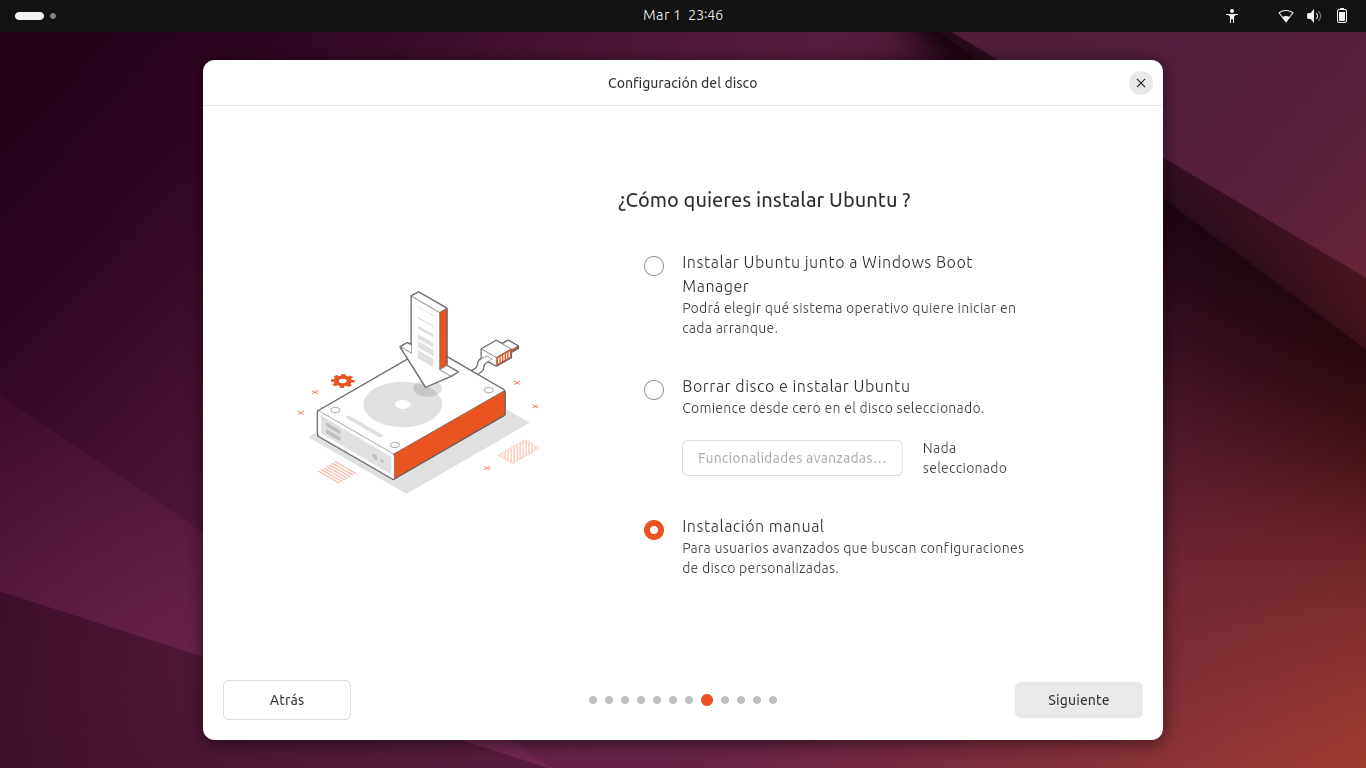
\includegraphics[width=0.85\linewidth]{./resources/images-ubuntu/ubuntu-tipo-instalacion.png}
        \caption{Elección de tipo de instalación}
\end{figure}

Luego nos preguntarán si queremos instalar la distribución o solo probarla (como he explicado antes). Como a nosotros nos interesa instalarla, seleccionamos “Instalar Ubuntu”, y luego a “Instalación interactiva”.    

\begin{figure}[H]
    \centering
    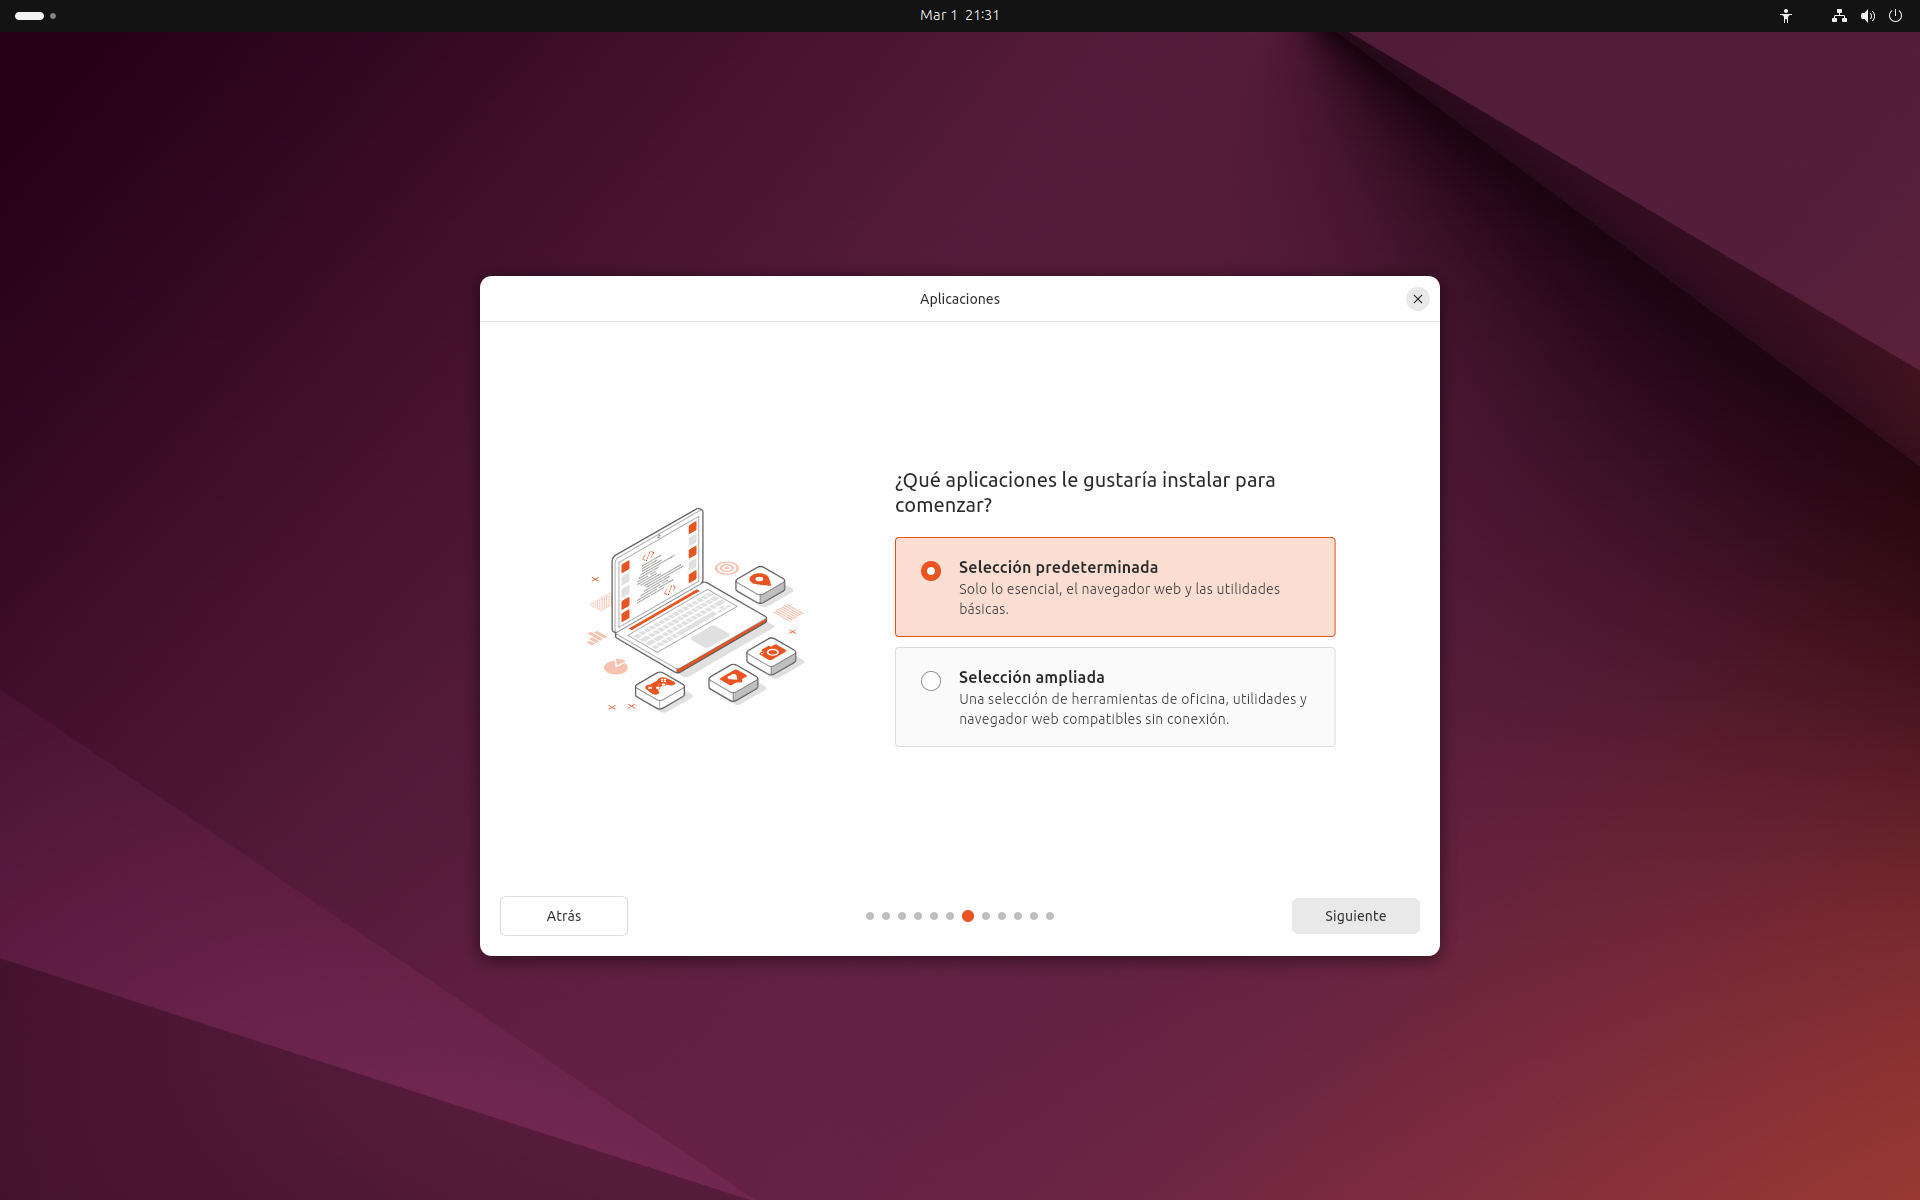
\includegraphics[width=0.85\linewidth]{./resources/images-ubuntu/ubuntu-selecciones-software.png}
    \caption{Selecciones de software}
\end{figure}

El siguiente paso es seleccionar el tipo de instalación. Si nos interesa una instalación mínima (pero suficiente), selecciona la predeterminada, si no, la ampliada. En mi caso, elijo la predeterminada, ya que no doy uso a las herramientas extra de la selección ampliada.

Tras esta pestaña, nos preguntarán si deseamos instalar software adicional (a veces privativo, como los drivers de NVIDIA). Parte de este software puede ser bastante útil, como los codificadores multimedia o los controladores Wi-Fi. Personalmente, he decidido instalarlos, pero depende de ti si quieres hacerlo o no.

\begin{figure}[H]
    \centering
    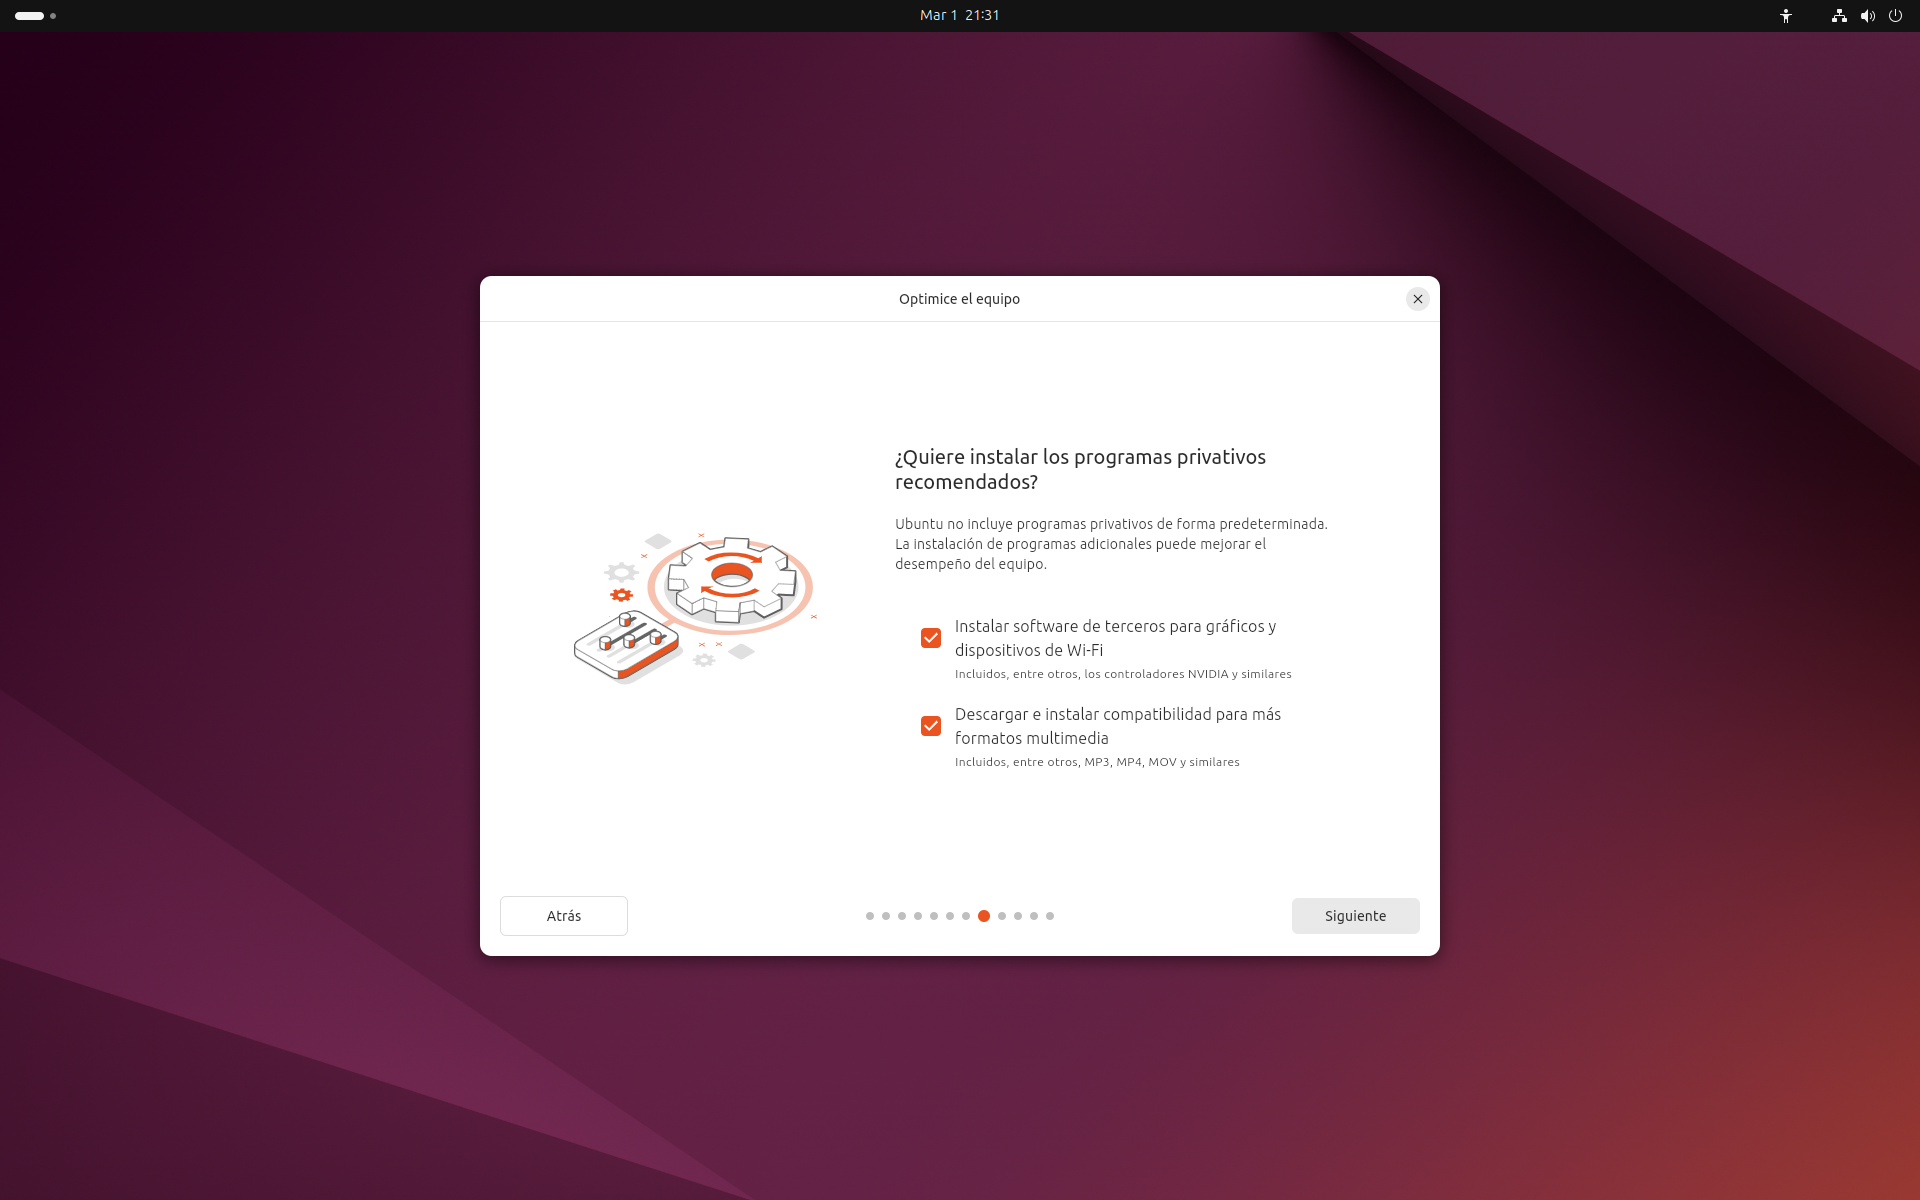
\includegraphics[width=0.85\linewidth]{./resources/images-ubuntu/ubuntu-drivers.png}
    \caption{Selección de drivers}
\end{figure}

\begin{figure}[H]
        \centering
        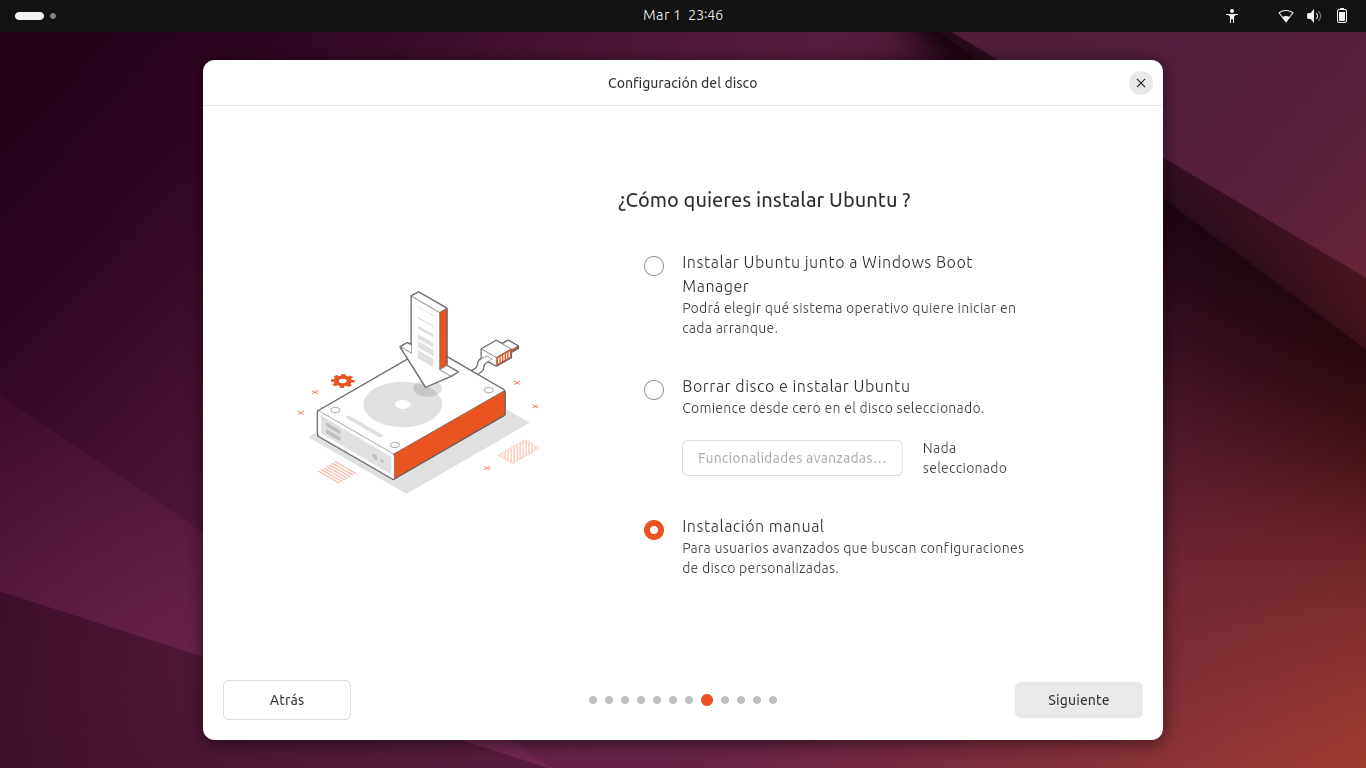
\includegraphics[width=0.85\linewidth]{./resources/images-ubuntu/ubuntu-instalacion-manual.png}
        \caption{Selección de instalación manual}
\end{figure}
    
Aquí viene una parte importante, la configuración de disco. Como hemos mencionado, el enfoque de este manual es para Dual Boot, así que veremos a fondo ese proceso. Sin embargo, si no quieres tener Dual Boot, lo tienes más fácil, porque puedes seleccionar “Borrar disco e instalar Ubuntu” y continuar normalmente con la instalación. Hacer esto eliminará por completo el contenido de tu disco duro.

Si quieres tener Dual Boot, selecciona “Instalación manual”, nos saldrá esta ventana:

\begin{figure}[H]
    \centering
    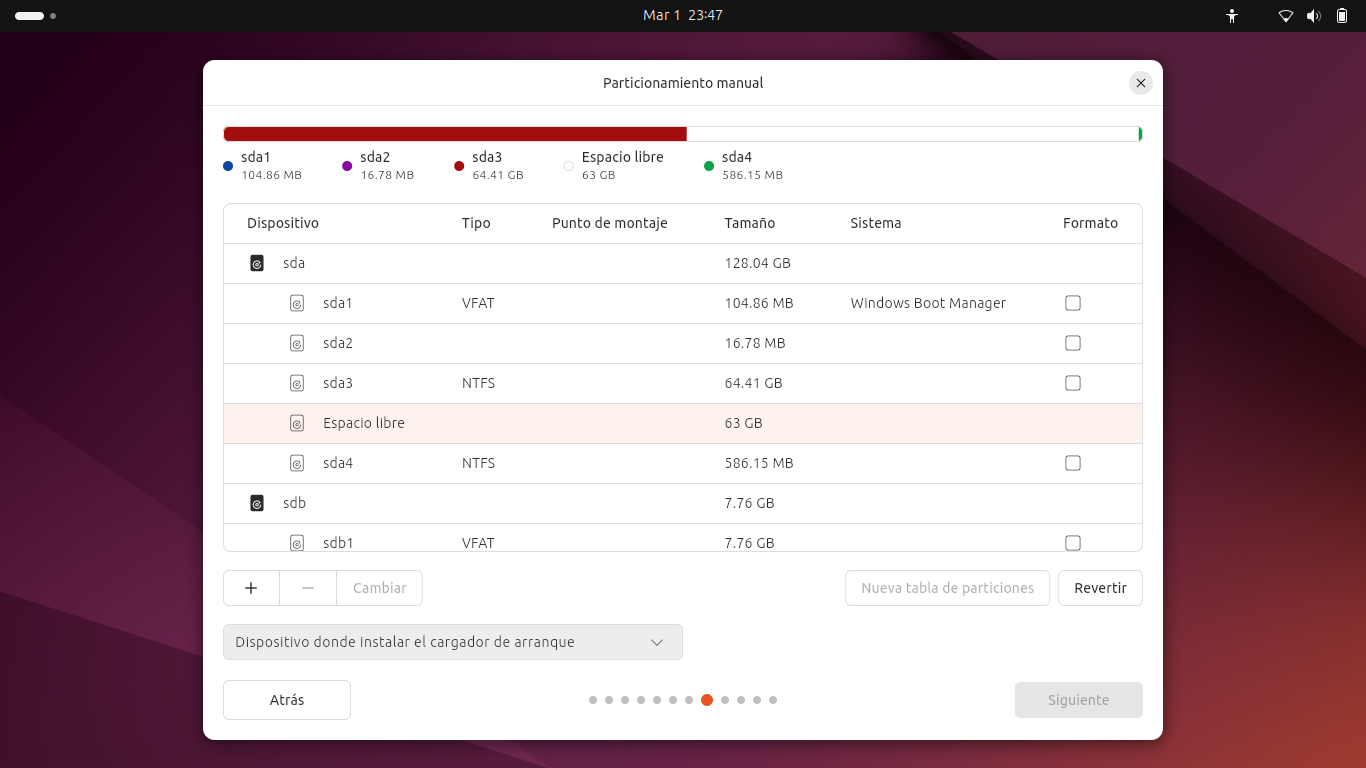
\includegraphics[width=0.85\linewidth]{./resources/images-ubuntu/ubuntu-particiones.png}
    \caption{Editor de particiones de Ubuntu}
\end{figure}

Estas son las particiones de tu sistema. Puede que esta lista te suene a la del administrador de disco, ya que te está mostrando precisamente lo mismo. Nos debería de salir, entre otras particiones, el espacio libre que hemos generado anteriormente. Es aquí donde instalaremos Ubuntu. Seleccionamos el espacio libre y le damos al botón “+”.

\begin{figure}[H]
    \centering
    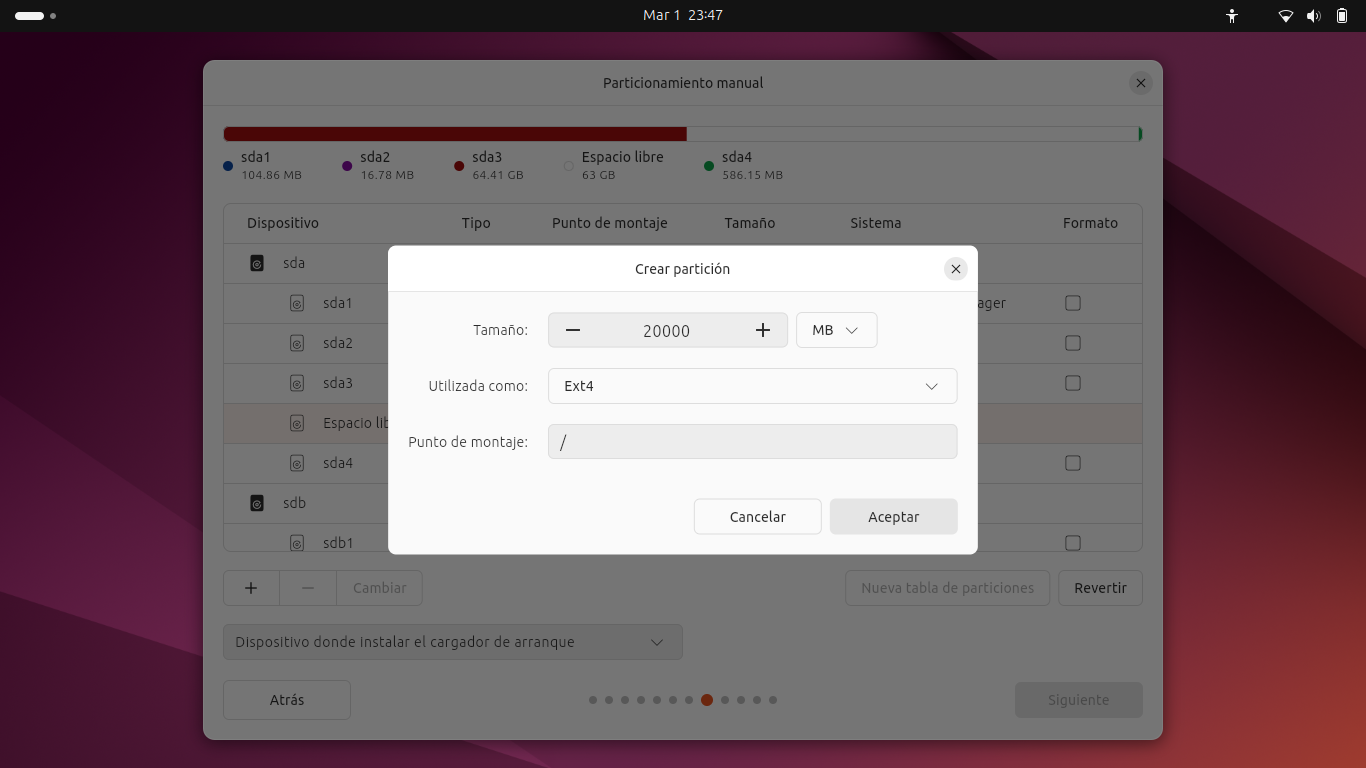
\includegraphics[width=0.85\linewidth]{./resources/images-ubuntu/ubuntu-crear-particion.png}
    \caption{Creación de partición con Ubuntu}
\end{figure}

En esta ventana vamos a asignar la partición (o particiones) de Ubuntu. Tenemos dos opciones: crear solo una partición, donde estará todo el sistema operativo, o crear dos, una para el sistema operativo y otra para tus ficheros personales (los directorios de usuario). Esta última opción resulta más útil y segura, ya que estamos separando nuestros ficheros personales de los ficheros del sistema operativo. Además, puede ser conveniente si planeas cambiar de distribución de manera habitual. En esta guía, usaré la segunda forma:

La primera partición será la del sistema operativo. Con 30 GB suele ser más que suficiente si no planeas instalar una cantidad excesiva de paquetes (nota: en la captura pongo 20 porque el espacio de la máquina virtual no era muy grande). Como formato dejamos Ext4 y nos aseguramos de que el punto de montaje sea root (/).

\begin{figure} [H]
    \centering
    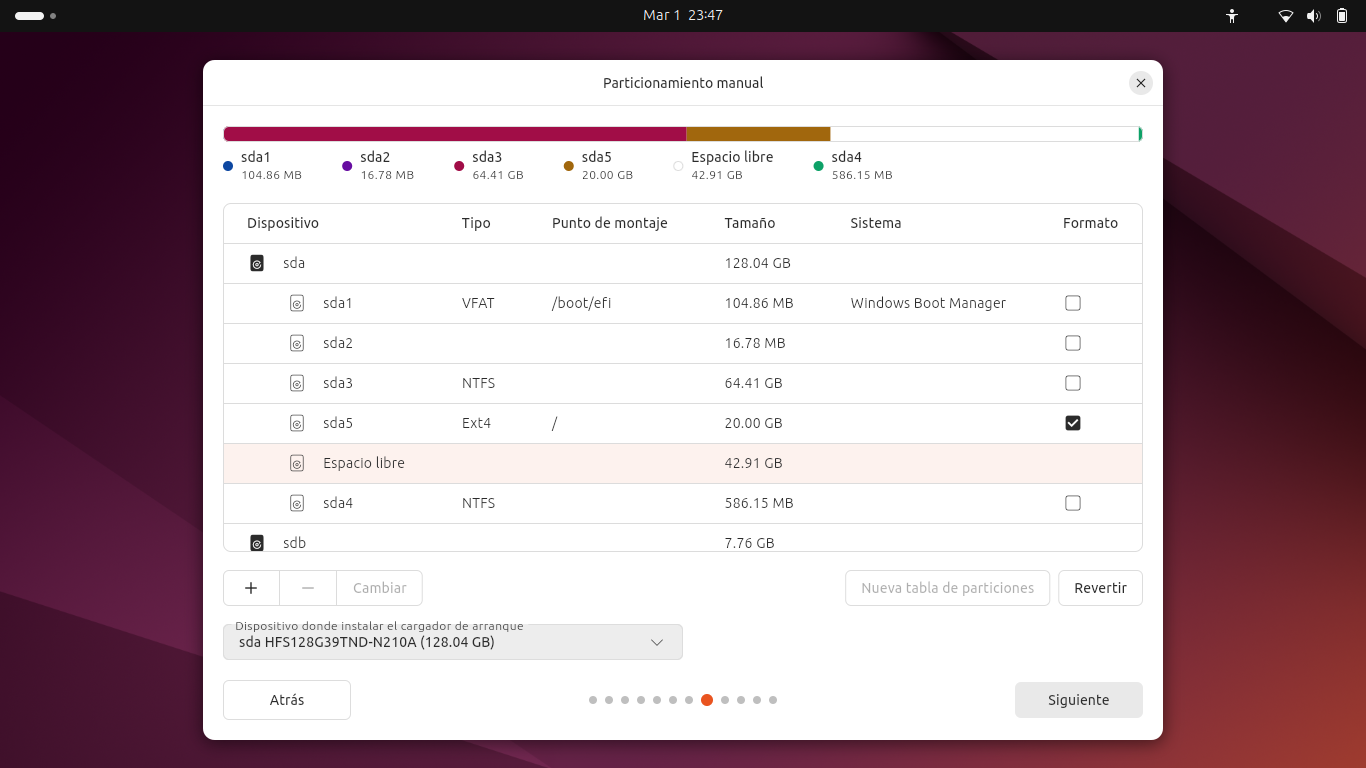
\includegraphics[width=0.85\linewidth]{./resources/images-ubuntu/ubuntu-root-creado.png}
    \caption{Partición root creada}
\end{figure}

Si hemos creado la partición correctamente, nos saldrá en la lista, junto con el espacio libre restante. El espacio libre restante será el de la partición de nuestros ficheros personales. Repetimos el proceso: seleccionamos el espacio libre, le damos a “+”, asignamos el espacio restante, usamos como formato Ext4, y ahora, el punto de montaje será en /home.

Solo falta una partición que configurar: la de GRUB, el bootloader. GRUB tiene que estar en la misma partición en la que se encuentra Windows Boot Manager.

\begin{figure}[H]
    \centering
    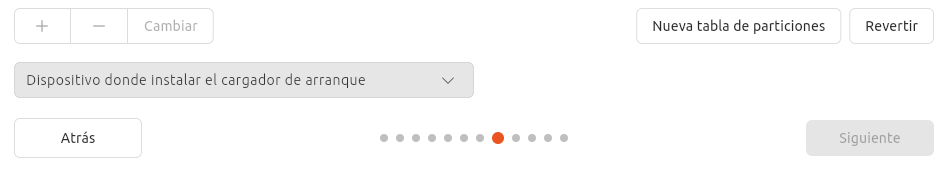
\includegraphics[width=0.85\linewidth]{./resources/images-ubuntu/ubuntu-selector-arranque.png}
    \caption{Selector de partición de arranque}
\end{figure}

Para seleccionar la partición basta con darle clic a “Dispositivo donde instalar el cargador de arranque”, y seleccionar el dispositivo donde se encuentran tus particiones (probablemente sda).

La partición de Windows Boot Manager debería quedar así (fíjate cómo el punto de montaje de la partición de Windows Boot Manager es ahora /boot/efi):

\begin{figure}[H]
    \centering
    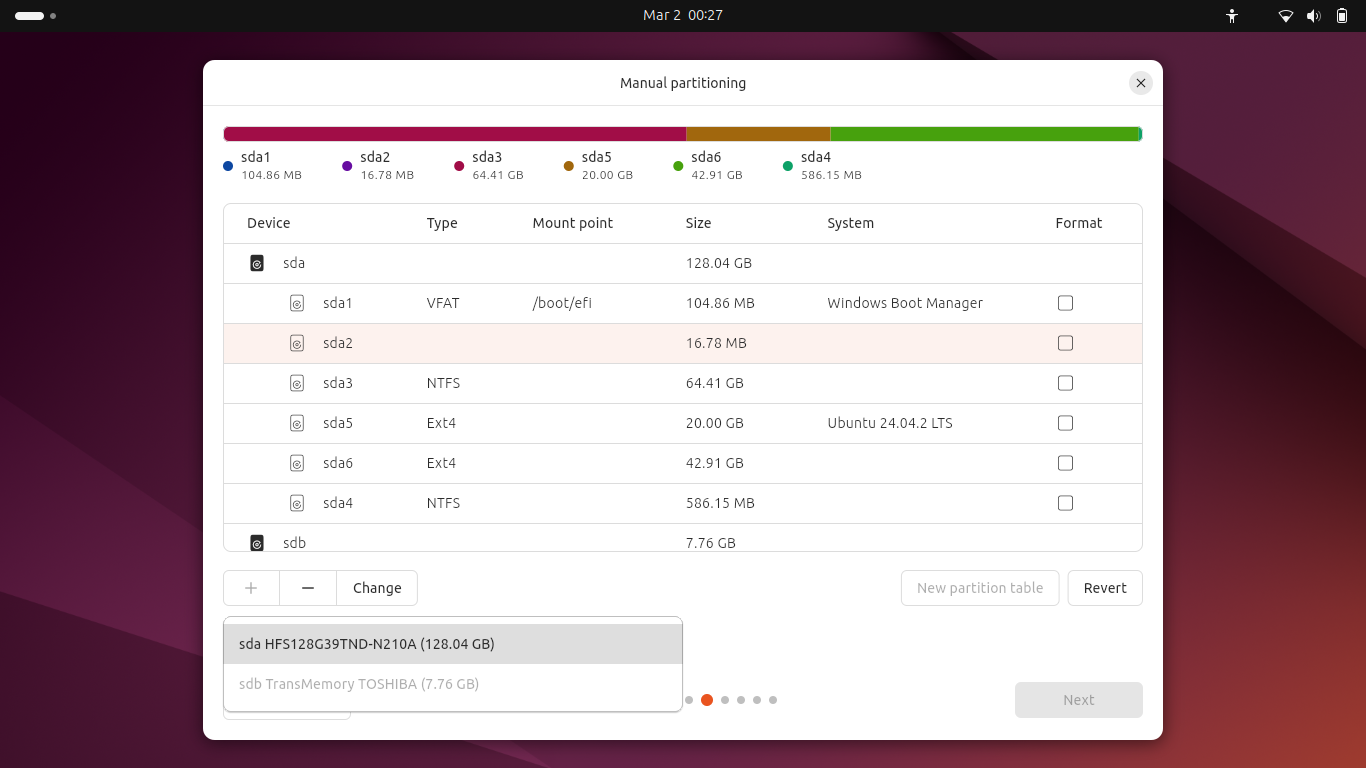
\includegraphics[width=0.85\linewidth]{./resources/images-ubuntu/ubuntu-arranque-elegido.png}
    \caption{Unidad de arranque elegida}
\end{figure}

Una vez creadas las particiones correctamente, podemos pasar a un paso más sencillo, el de crear un usuario para el sistema:

\begin{figure}[H]
    \centering
    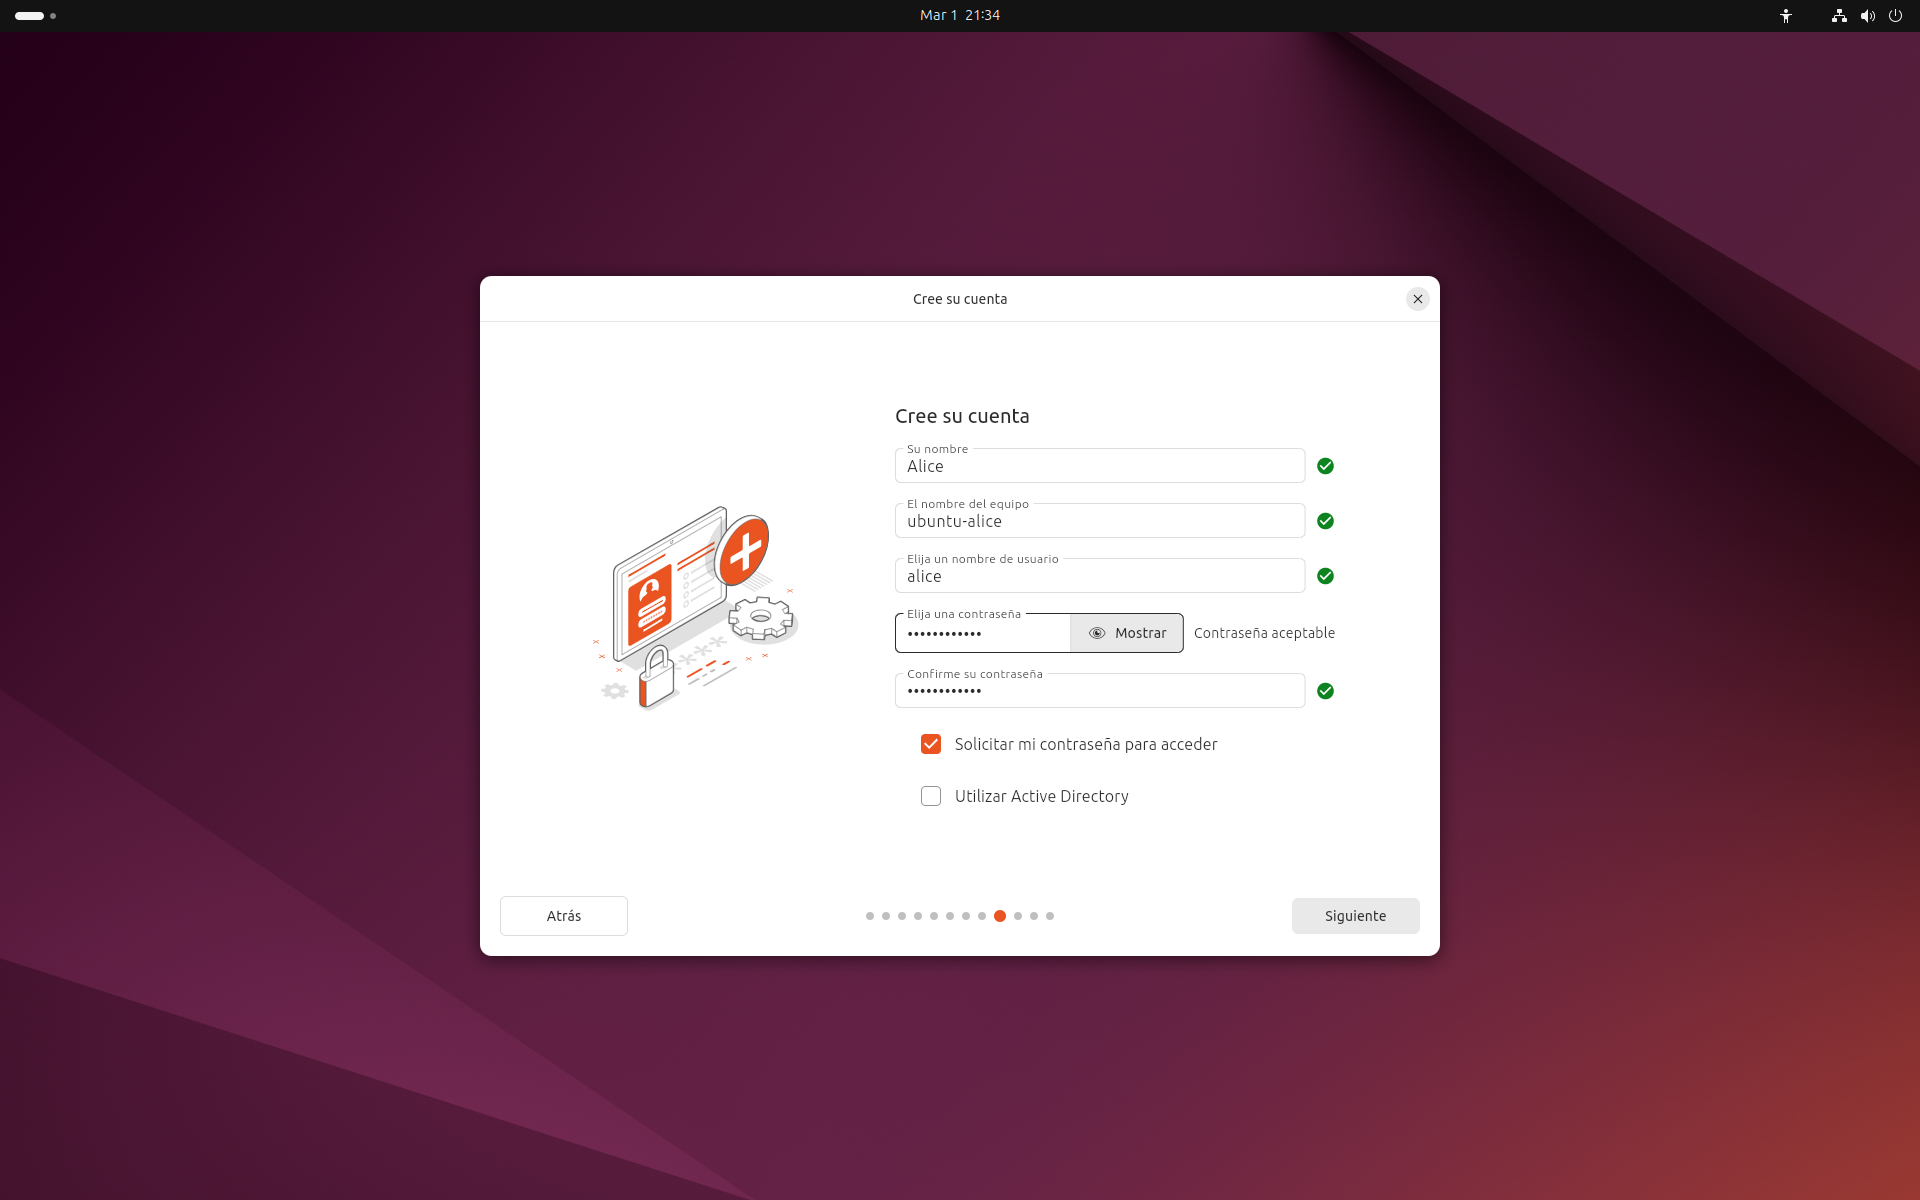
\includegraphics[width=0.85\linewidth]{./resources/images-ubuntu/ubuntu-crear-usuario.png}
    \caption{Ventana de configuración de usuario}
\end{figure}

No activo Active Directory porque no es necesario en absoluto. Active Directory es una forma de conectar tu distribución de Ubuntu con un sistema Windows, pero existen otras maneras y de todas formas este proceso es irrelevante para la instalación.

\begin{figure}[H]
    \centering
    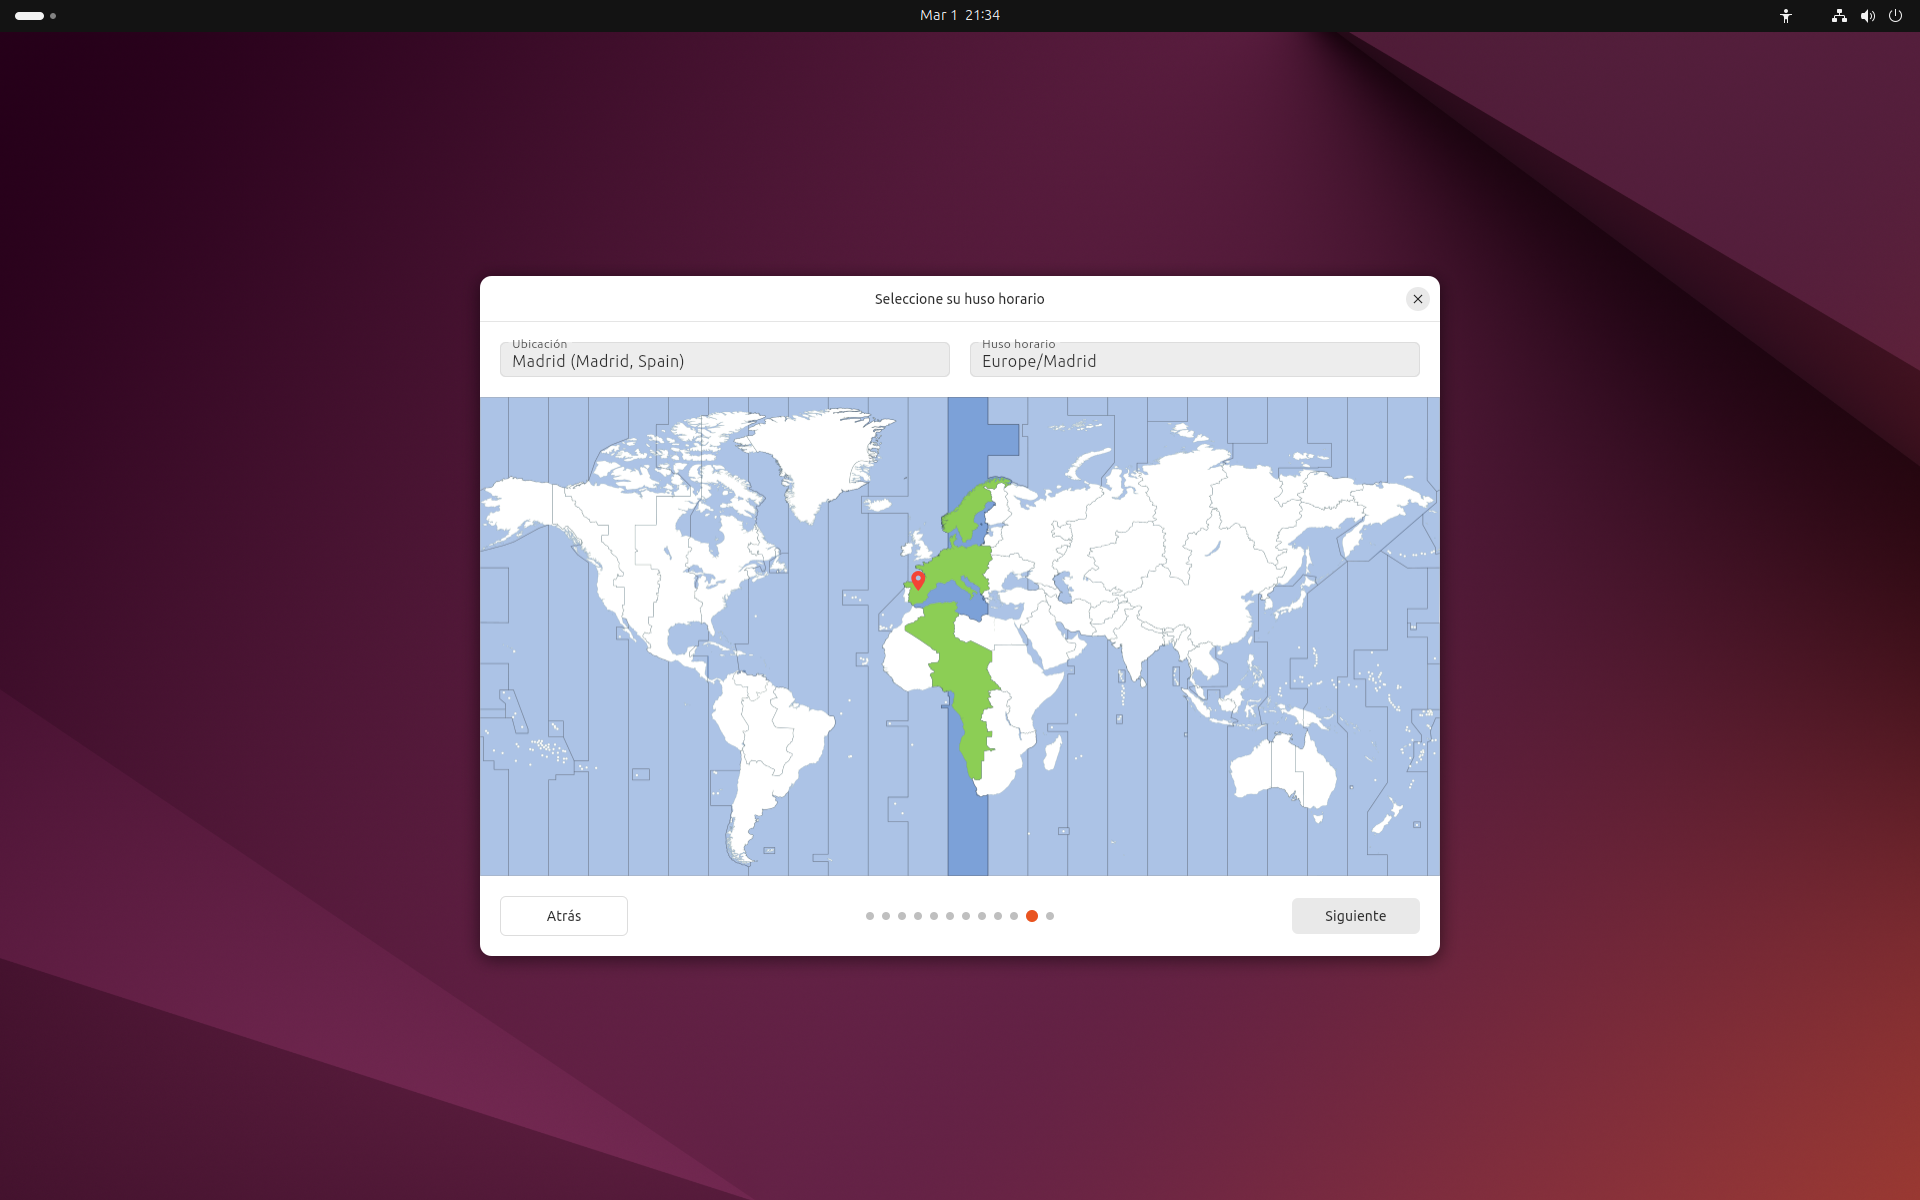
\includegraphics[width=0.85\linewidth]{./resources/images-ubuntu/ubuntu-zona-horaria.png}
    \caption{Selección de zona horaria}
\end{figure}

Después seleccionamos nuestra zona horaria, y al hacerlo, nos saldrá una última ventana antes de la instalación, para confirmar las configuraciones de instalación. Comprobamos que todo está correcto, y le damos al botón de “Instalar”.

\begin{figure}[H]
    \centering
    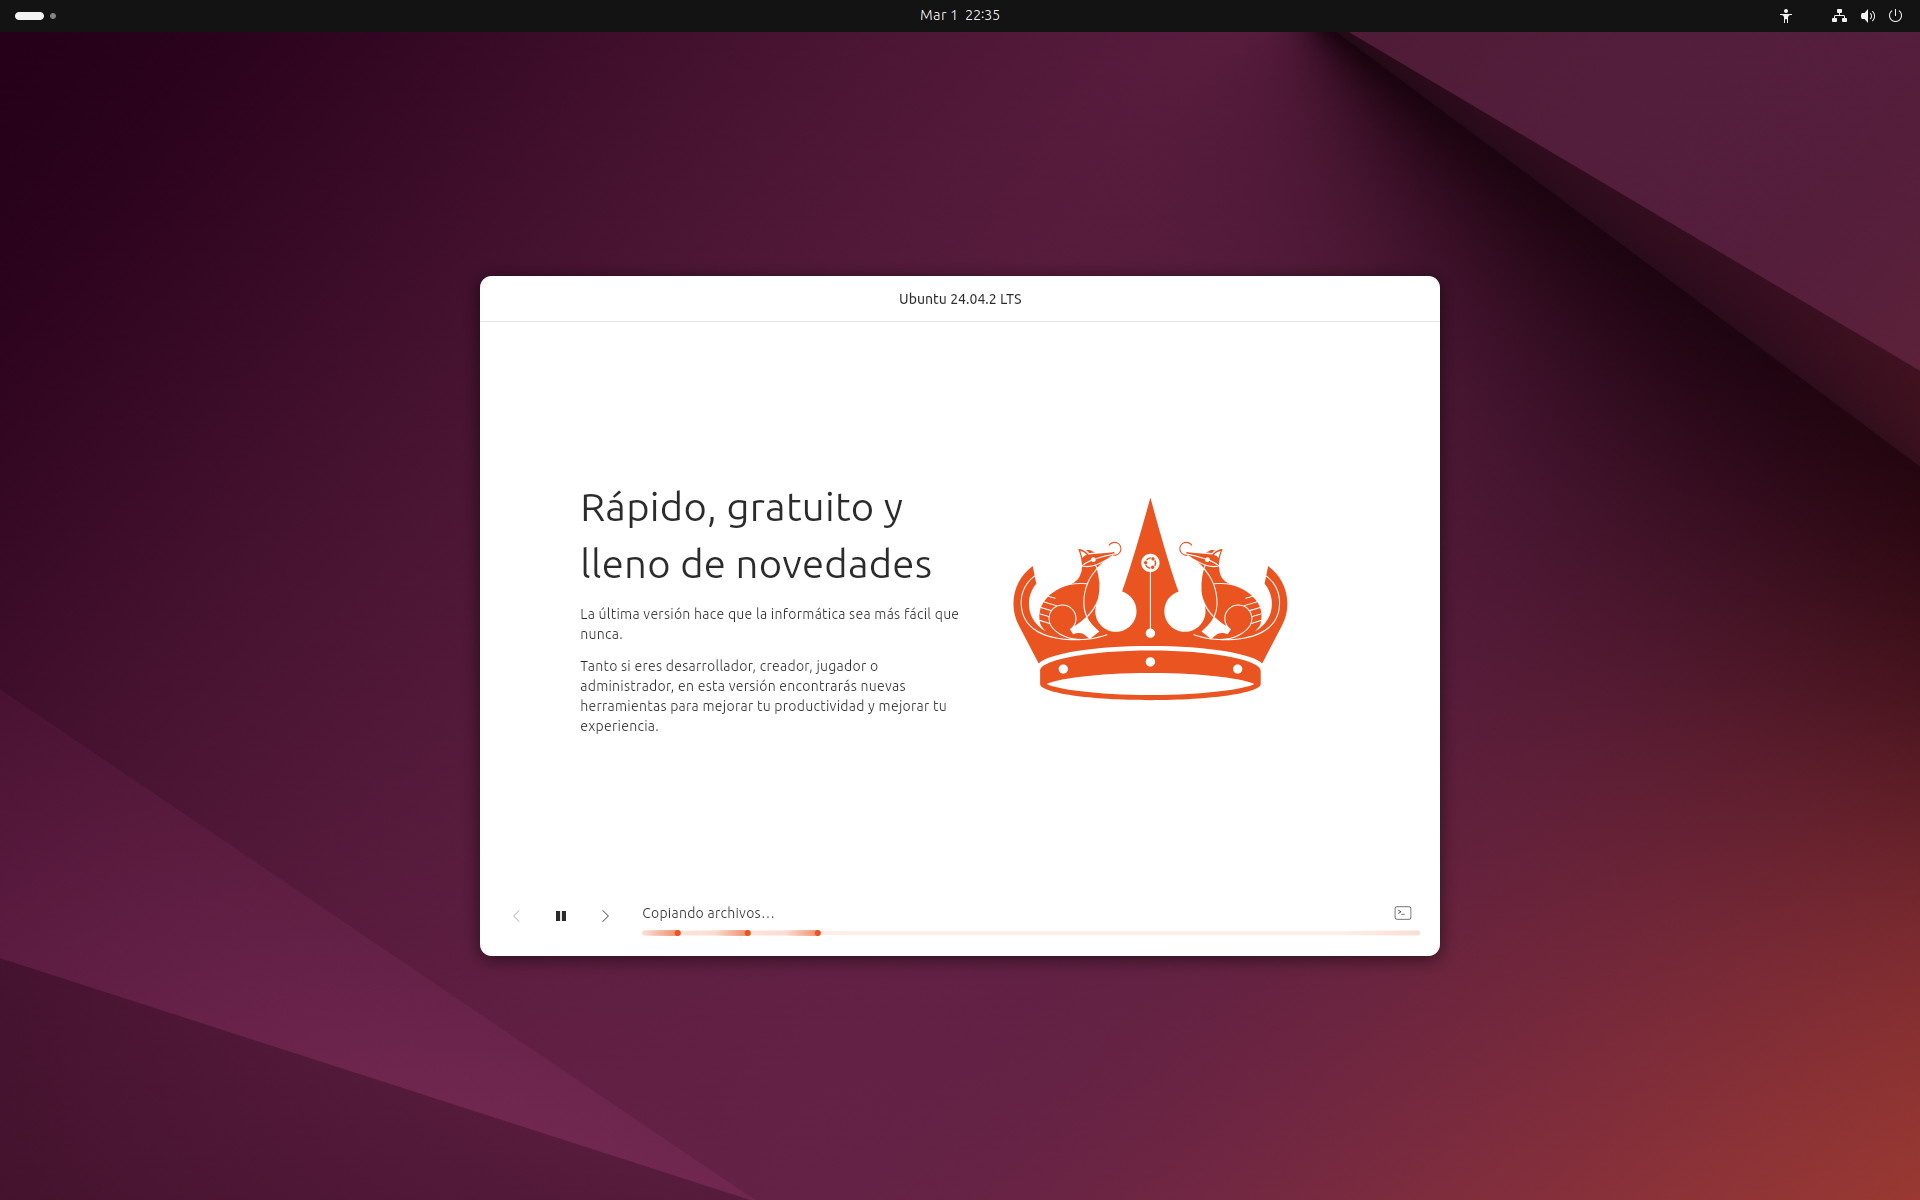
\includegraphics[width=0.85\linewidth]{./resources/images-ubuntu/ubuntu-comienzo-instalacion.png}
    \caption{Proceso de instalación de Ubuntu}
\end{figure}

A partir de aquí, hemos terminado con la configuración para la instalación. De lo que queda se encargará el instalador. Si le das al botón de la terminal, podrás ver cómo se están instalando paquetes y dependencias para el sistema operativo. Ten en cuenta que este proceso puede durar un buen rato, y que cabe la posibilidad de que se atasque durante varios minutos en un mismo paso. No te preocupes y ten paciencia, ya casi hemos terminado.

\chapter{GRUB}

Cuando la instalación termine, Ubuntu te preguntará si deseas seguir probando Ubuntu o si quieres reiniciar el ordenador. Si le damos a “Reiniciar” y retiramos el medio de instalación, es posible que el ordenador arranque en Windows, como si no hubiera pasado nada. No te preocupes, es normal. De hecho, es una buena señal, ya que no hemos perdido acceso a Windows y nuestros datos están seguros. Sin embargo, si intentamos arrancar el sistema en Ubuntu, rápidamente nos daremos cuenta de que no podemos. Esto se debe a que, si bien GRUB está instalado, no está activado como bootloader por defecto.

Para solucionar esto, abre el menú de inicio de Windows, escribe “cmd”, y ejecútalo con permisos de administrador. Esto abrirá la terminal de comandos de Windows, PowerShell.

Para solucionar este problema necesitamos ejecutar el siguiente comando:

\begin{tcolorbox-code}
\begin{lstlisting}
bcdedit /set "{bootmgr}" path \EFI\ubuntu\grubx64.efi
\end{lstlisting}
\end{tcolorbox-code}

Esencialmente, este comando cambia el bootloader por defecto que se ejecuta en la partición de Windows Boot Manager. La dirección que introducimos después del argumento “path” es precisamente la de GRUB. No te preocupes, al ejecutar este comando no perderemos el acceso a Windows. Como se ha mencionado anteriormente, GRUB es un bootloader dinámico. Nos da acceso a Ubuntu pero también a Windows.

Si ahora reiniciamos el ordenador, tras ejecutar el comando, nos saldrá un menú muy parecido a este:

\begin{figure}[H]
    \centering
    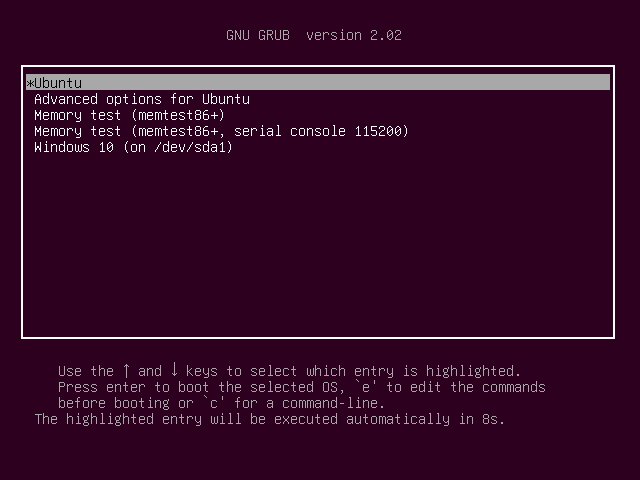
\includegraphics[width=0.85\linewidth]{./resources/images-ubuntu/grub-windows-ubuntu.png}
    \caption{Menu de GRUB con Windows y Ubuntu}
\end{figure}

Desde aquí podemos acceder tanto a Ubuntu como a Windows. Comprobamos que efectivamente podemos, y con esto la instalación de Ubuntu ha terminado.

\chapter{Conclusión}

Como hemos podido ver, instalar Ubuntu no es complicado, ni siquiera con Dual Boot. Los pasos suelen ser muy parecidos entre distribuciones y no tienen mucho misterio. Ahora que tienes Ubuntu instalado en tu ordenador, con Dual Boot, aprender a usar Linux será mucho más sencillo, ya que tienes tu propia distribución con el sistema operativo. No tengas miedo a usar la terminal, cargarte una distribución tan estable como es Ubuntu es cuanto menos complicado. Y ya para terminar, intenta acostumbrarte a la interfaz de GNOME (el gestor de ventanas que utiliza Ubuntu por defecto), ya verás como es bastante sencilla de usar, aunque la magia de Linux realmente se encuentra en la terminal. Ahí podrás sacarle mucho partido al sistema operativo.

\textbf{¡Gracias y mucha suerte!}

\end{document}
